\documentclass[ngerman,11pt,parskip=half] {scrartcl}

\usepackage{babel}

%
% Schrift
%
\usepackage[T1]{fontenc}
\usepackage{textcomp}
\usepackage[utf8]{inputenc}
\usepackage{eurosym}% 1 \euro oder \EUR{1}

\usepackage{helvet}
\renewcommand{\ttdefault}{pcr} %typewriter default font
\renewcommand{\familydefault}{\sfdefault}

%
% Layout
%
\usepackage[textwidth=16cm,head=4cm,bottom=3cm,a4paper]{geometry}
\usepackage{scrlayer-scrpage}
\pagestyle{scrheadings}
%\chead{}\ihead{}\ohead{}
\cfoot{}\ifoot{\footnotesize \currfilepath}\ofoot{\footnotesize Seite \pagemark~von \pageref*{LastPage}} % pageref* -> kein klickbarer Link
\renewcommand*{\footfont}{\normalfont}%nicht kursiv

\usepackage{lastpage}
\usepackage[table]{xcolor}
\usepackage{multicol}
\usepackage{rotating}
\usepackage{graphicx}
\usepackage{setspace}
\linespread{1.1}%zeilenabstand default global
\usepackage{array}
\usepackage{longtable}
\usepackage{ltxtable}
\setlength\LTleft{0pt}
\setlength\LTright\fill
\usepackage{tikz}
\usepackage{ctable}
\newcommand{\otoprule}{\midrule[\heavyrulewidth]}
\usepackage{hhline}
\usepackage{cals}
\usepackage{enumitem}% f"ur besseres itemize
\setitemize{label=\textminus,itemsep=0pt,topsep=0.5ex,after=\vspace{\baselineskip}}
\usepackage{float} %bilderpositionierung
%\usepackage{textgreek}
\usepackage{sansmath}
\usepackage{listings}
\lstset{basicstyle=\footnotesize\ttfamily,breaklines=true}
\lstset{framextopmargin=50pt,frame=bottomline}

% Funktion zum Generieren des Dateipfades. Kann leider nicht den absoluten Pfad finden...
\usepackage{currfile}

% Zeit
\usepackage{datetime}

%
% Funktionen
%
% fettes rotes todo
\newcommand {\todo} {\textbf{\color{red} todo\ }}
% Gr"o"se eines Oszillogramms
\newcommand {\tscopesize}{12cm}

% Links, Querverweise, Titel
\usepackage[
  colorlinks=true,
  linkcolor=black,
  urlcolor=black,
  pdftitle={Schaltungsbeschreibung}, %PDF Beschreibung
  allcolors=black,
]{hyperref} %immer zum Schluss

%
% Dokument
%
\begin{document}
\sansmath

% Titelseite

\thispagestyle{empty}

\mbox{}\\[2cm]%absolute L"ange

\textbf{\huge
Saba Webradio Hardware
}

\vfill

\hspace{1cm}\begin{tabular}{ll}
Autor: & 		Martin Wagner, DL2WAG\\
Dokumentart:&   Schaltungsbeschreibung, Messungen\\
Datum:&         \today \enspace \currenttime
\end{tabular}




\vfill
\begin{minipage}[t]{\textwidth}
\begin{spacing}{1.2}%zeilenabstand lokal 
  \begin{tabular}{p{.1\textwidth} p{.2\textwidth}  p{.6\textwidth}}%
  Version & Datum & Bemerkung        \\
  \hline  
  \hspace{.02\textwidth} 1  & 05.06.2022 & Neu   \\  
  \end{tabular}
\end{spacing}
\end{minipage}


\mbox{}\\[2cm]%absolute L"ange

% Inhaltsverzeichnis

\newpage
\tableofcontents

% eigentliches Dokument

\newpage

\section{Saba Webradio} \label{sec:sabawebradio}

Das Saba Webradio erweitert ein Saba Automatic Radio um die folgenden Funktionen:
\begin{itemize}
\item W-Lan Webradio
\item Steuerung von Automatik und Lautst"arke per Webinterface, MQTT, IR Fernbedienung ...
\item Steuerung des Webradio per Radio Automatiktasten
\end{itemize}
Es kann direkt auf die Anschlussbuchse f"ur die Fernbedienung aufgesteckt werden. Kompatibel sind mind. das Meersburg und Freiburg 6-3D. Am Ger"at selbst sind keine Modifikationen notwendig (aber empfehlen). Der Audioausgang des Webradio wird mit dem TA Eingang des Radios verbunden und kann durch Wahl des zugeh"origen Eingangs am Radio verwendet werden.

\begin{figure}[H]
\centering
\begin{tikzpicture}
.-     \node[anchor=south west,inner sep=0] at (0,0) {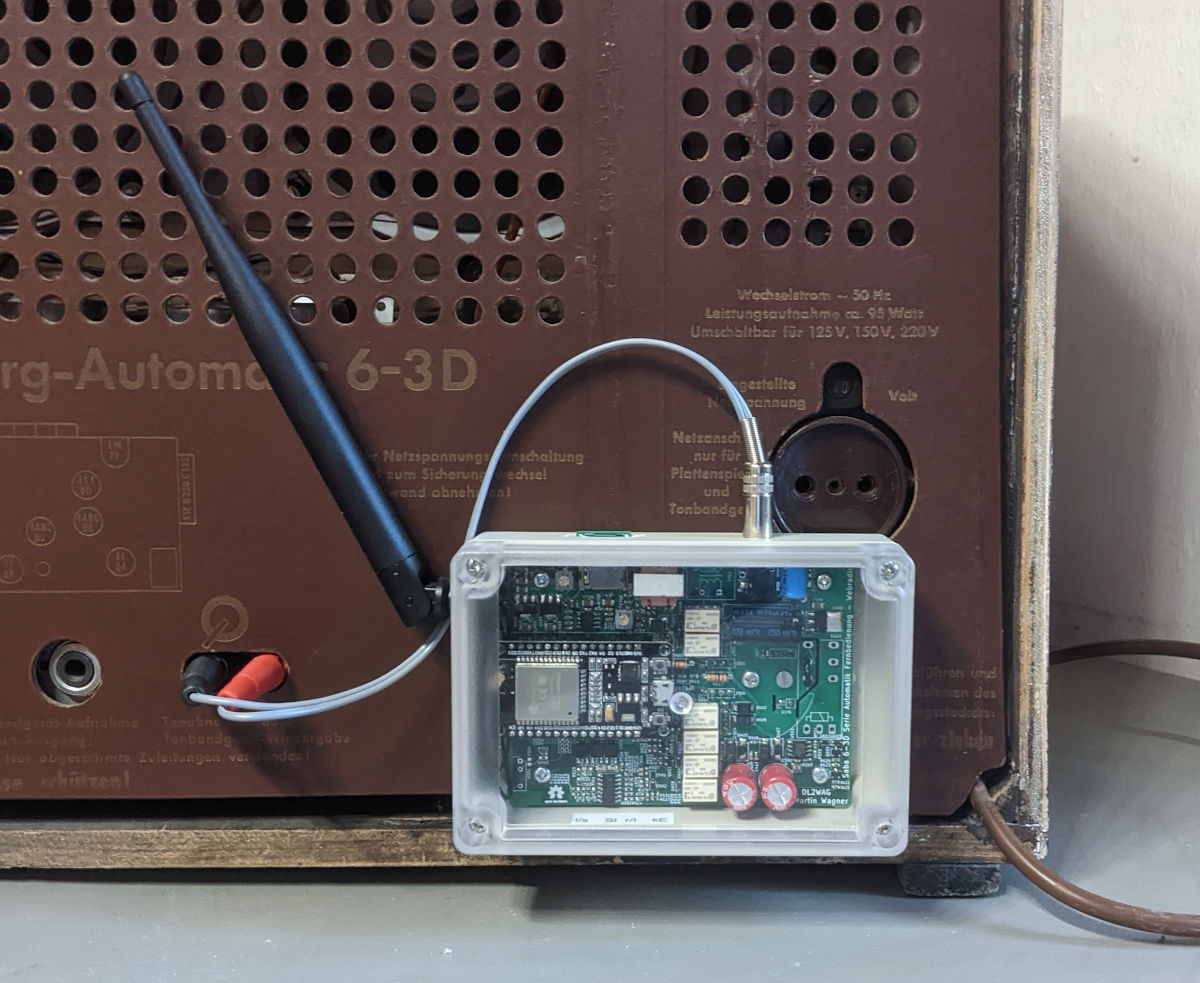
\includegraphics[width=.7\textwidth]{komplett.jpg}};
\end{tikzpicture}
\caption{Fertig montiertes Saba Webradio} \label{fig:1}
\end{figure}

Das Webradio basiert auf dem ESP32-Radio Projekt von Ed Smallenburg: \url{https://github.com/Edzelf/ESP32-Radio}.

Hardware: \url{https://github.com/martin-wagner/saba-6-3d-fernbedienung-hw}\\
Software: \url{https://github.com/martin-wagner/ESP32-Radio}


\section{Empfohlene Modifikationen} \label{sec:mod}

\subsection{Magisches Auge} \label{sec:mod:magischesauge}

Wird h"aufig die Webradiofunktion verwendet, sollte das magische Auge im TA Betrieb deaktiviert werden. Bei neueren Saba Ger"aten ist dies ab Werk der Fall, bei "alteren wie dem 6-3D wie folgt modifizieren:

\begin{figure}[H]
\centering
\begin{tikzpicture}
     \node[anchor=south west,inner sep=0] at (0,0) {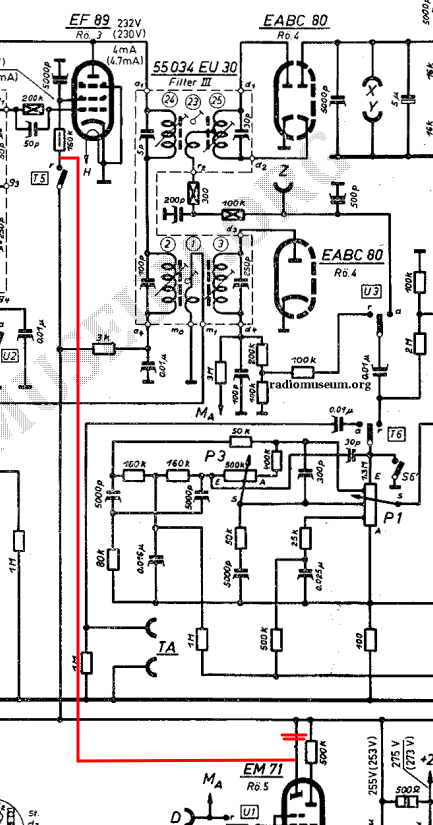
\includegraphics[width=6cm]{auge.png}};
\end{tikzpicture}
\caption{Schaltungsvorschlag} \label{fig:1}
\end{figure}

Um ein ggf. neu gekauftes Auge zu schonen kann bei diesem Umbau auch direkt ein Poti 1\,W 50\,kOhm in Serie eingeschleift werden. Je niedriger die Helligkeit eingestellt wird desto h"oher ist die Lebensdauer des Auges. Ohne Widerstand ist bei der verwendeten EM71 ein Abnutzungseffekt bereits nach wenigen Betriebsstunden (!!!) sichtbar.

\subsection{Erkennung TA aktiv} \label{sec:mod:erkennungta}

Das Webradio hat keine M"oglichkeit zu erkennen ob gerade normales Radio oder Webradio aktiv ist. Der Webradio Stream ist daher immer eingeschalten. Abgesehen von unn"utzer Daten"ubertragung f"uhrt die W-Lan Kommunikation zu St"orungen im Radioempfang bei schw"acheren Sendern. Soll dies vermieden werden kann das "`TA Aktiv"' Signal von der Gl"uhlampe der TA Taste abgegriffen und an die Fernbedienungsbuchse verdrahtet werden. Hierf"ur wird der freie Kontakt "`11"' verwendet.

\begin{figure}[H]
\centering
\begin{tikzpicture}
     \node[anchor=south west,inner sep=0] at (0,0) {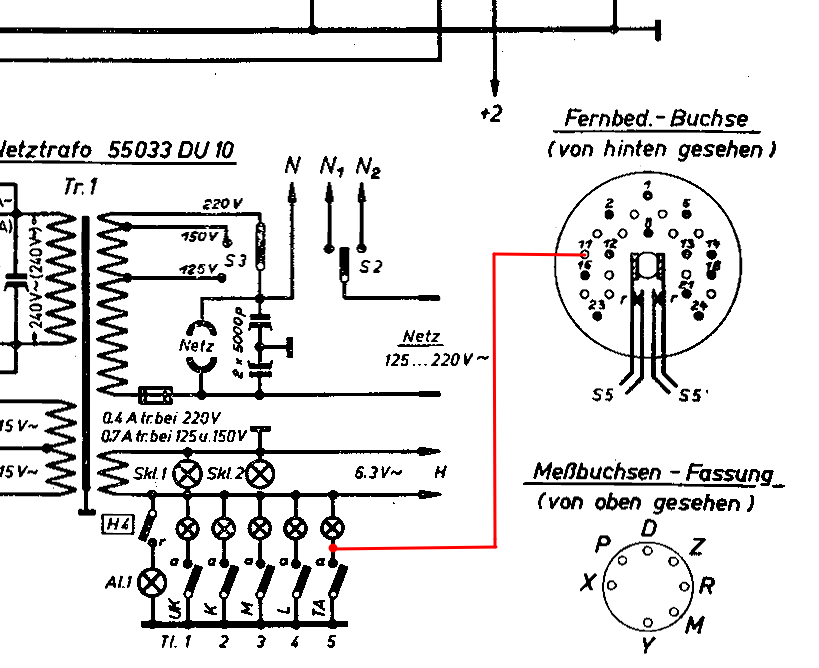
\includegraphics[width=7cm]{ta_erkennung.png}};
\end{tikzpicture}
\caption{Schaltungsvorschlag} \label{fig:1}
\end{figure}

Unbenutzte Kontakte sind leer, daher muss ein Kontaktstift aus einem Schlachtger"at entfernt werden. Alternativ kann die 230\,V Wechselschaltung geopfert und einer der zugeh"origen Kontaktstifte versetzt werden.

\begin{itemize}
\item Leitung abl"oten
\begin{figure}[H]
\centering
\begin{tikzpicture}
     \node[anchor=south west,inner sep=0] at (0,0) {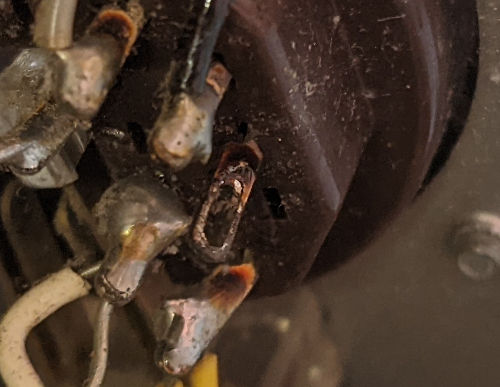
\includegraphics[width=8cm]{stecker1}};
\end{tikzpicture}
\caption{Kontakt ohne Leitung} \label{fig:1}
\end{figure}
\item L"ot"ose reinigen und geradebiegen
\begin{figure}[H]
\centering
\begin{tikzpicture}
     \node[anchor=south west,inner sep=0] at (0,0) {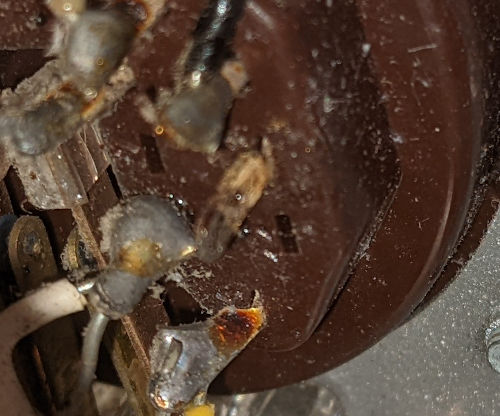
\includegraphics[width=8cm]{stecker2}};
\end{tikzpicture}
\caption{Kontakt gerade} \label{fig:1}
\end{figure}
\item Feder zur Ger"ate Au"senseite herausschieben
\begin{figure}[H]
\centering
\begin{tikzpicture}
     \node[anchor=south west,inner sep=0] at (0,0) {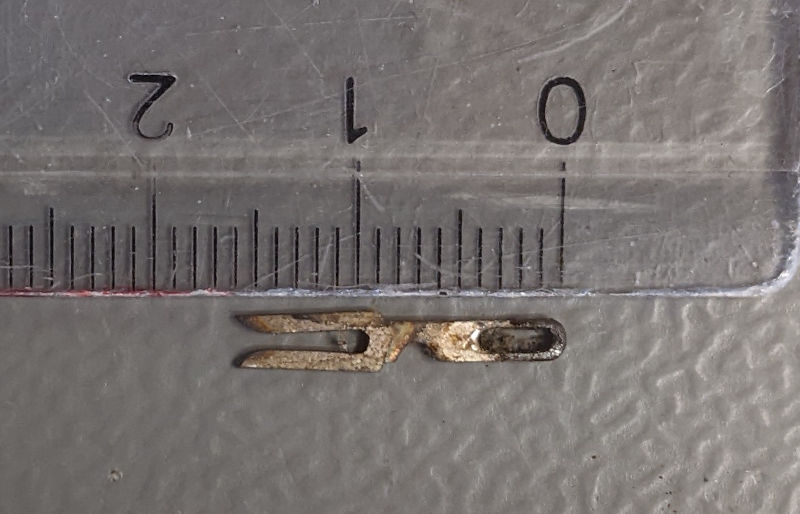
\includegraphics[width=8cm]{stecker4}};
\end{tikzpicture}
\caption{Kontaktstift} \label{fig:kontakt-feder}
\end{figure}
\item Umsetzen und Schaltung nach Vorgabe herstellen
\begin{figure}[H]
\centering
\begin{tikzpicture}
     \node[anchor=south west,inner sep=0] at (0,0) {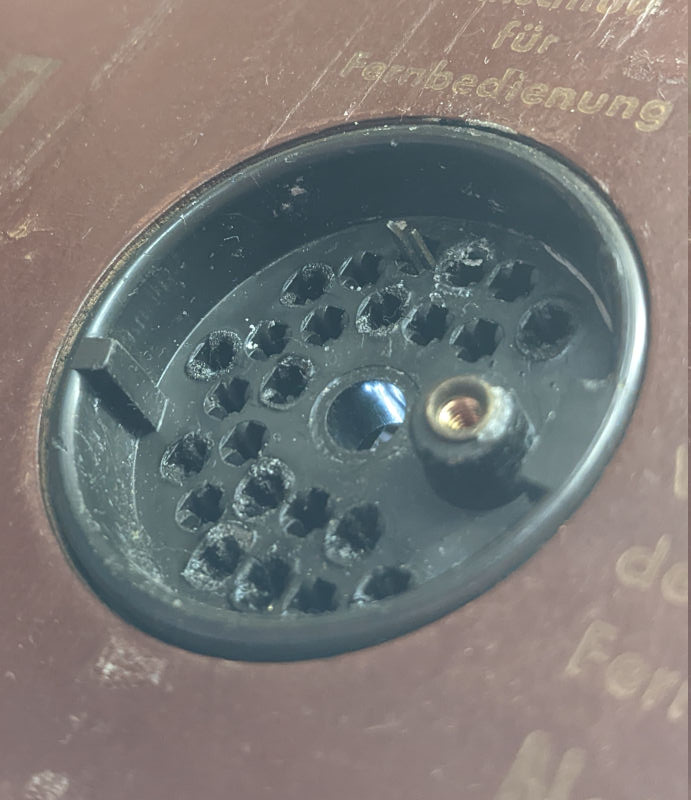
\includegraphics[width=8cm]{stecker3}};
\end{tikzpicture}
\caption{Kontakt an neuer Position} \label{fig:1}
\end{figure}
\begin{figure}[H]
\centering
\begin{tikzpicture}
     \node[anchor=south west,inner sep=0] at (0,0) {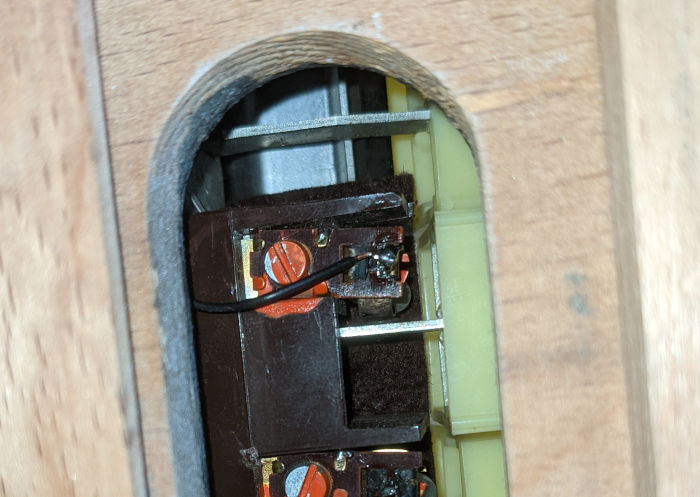
\includegraphics[width=8cm]{lampe}};
\end{tikzpicture}
\caption{Anschluss an Lampenfassung} \label{fig:1}
\end{figure}
\end{itemize}


\section{Aufbau} \label{sec:aufbau}

Die Schaltung ist auf drei Platinen aufgebaut:
\begin{itemize}
\item Anschlussstecker Radio
\item Webradio Steuerplatine
\item ESP32 Aufsteckplatine
\end{itemize}

Der Anschlussstecker wird "uber eine 2,54\,mm Stiftleiste mit der Steuerplatine verbunden. Dies erm"oglicht ein Anpassen des Steckers auf Ger"atetypen mit anderer Buchse. Das ESP32 wird einfach auf die Basisplatine aufgesteckt und kann bei Bedarf entfernt werden.

\subsection{Material} \label{sec:aufbau:material}

Deutsche Distris versenden nur an Kunden mit Steuernummer (Firma). Internationale Distris machen keine Unterscheidung. Ich habe daher alles was \emph{Reichelt} nicht hat bei Digikey in den USA bestellt. Alle Bauteile mit Herstellervorgabe, z.B. \emph{WE}, k"onnen von einem beliebigen Hersteller kommen, solange die Kenndaten eingehalten werden.

Folgendes Material wird ben"otigt:
\begin{itemize}
\item Bauteile nach "`stueckliste.csv"' f"ur Anschlussstecker und Basisplatine. Bauteile mit Markierung \emph{NP} (No Placement) werden i.d.R. nicht ben"otigt (siehe Rest der Anleitung).\\
Die erste H"alfte der Liste sind alle Bauteile einzeln mit Index, die zweite H"alfte die Summe der Bauteile.
\item Jeweils eine Platine Anschlussstecker und Steuerung. Anschlussstecker -- 2lagig, Steuerung -- 4lagig. Bestellen z.B. bei \emph{JLC-PCB}, die Platinen sind kleiner als 10\,cm x 10\, cm. Falls man Reflow L"oten will den Stencil gleich mitbestellen. Auf der Unterseite sind keine Bauteile.
\item 2x ESP32 DOIT-DEVKITV1-ESP32-WROOM-32. Bestellen z.B. bei Ebay. Es gibt ESP32 Boards auch mit zwei Pins mehr, daher Pinbelegung vergleichen! Der zweite ist  notwendig falls man vermutet den ersten zerst"ort zu haben.
\item VLSI VS1053B. Bestellen z.B. bei Digikey (teuer) oder Ebay direkt aus China (Risiko gef"alschte Chips zu bekommen). Ich habe bei Ebay bestellt und meine Lieferung war OK.
\item 2x Buchsenleiste 2,54mm 15pol, f"ur ESP32
\item 6x Stiftleiste 2,54mm 4pol, $l \geq 20mm$, f"ur Verbindung der beiden Platinen
\item Ausgangstrafo 600 Ohm, 1:1. Ebay, Suche nach \emph{transformer EI14}. Falls nicht zu bekommen kann auch ein anderer verwendet werden, siehe  \ref{sec:untersuchung:ausgangsuebertrager}.
\item Klinkenstecker 3,5\,mm + Audiokabel + 2x Bananenstecker.
\item Geh"ause Hammond RP1125C. Das exakt gleiche Geh"ause gibt es auch von anderen Herstellern.
\item Kunststoff- / Holzstab rund, $d=6\,mm$, ca. 5\,cm lang. Ein Bleistift funktioniert auch, bricht aber leicht ab.
\item Messingstab 3\,mm x 1,5\,mm, mind. ca. 30\,cm. Wenn man es bekommt ist 3\,mm x 1,2\,mm besser, ggf. geht auch 3\,mm x 1,0\,mm.
\item Ein Set SMD Widerst"ande 0603, wenn noch nicht vorhanden. Notwendig falls ein Widerstandswert angepasst werden muss. Ebay, Suche nach \emph{resistor kit 0603}.
\item Ggf. eine W-Lan Antenne.
\item Gut gef"ullte Teilekiste f"ur alles was ich vergessen habe.
\end{itemize}


\subsection{Anschlussstecker Radio} \label{sec:aufbau:anschlussstecker}

Wir brauchen:
\begin{itemize}
\item Platine
\item Messingstab
\item Holzstab
\end{itemize}

Aus dem Messingstab 13 Stifte mit je 15\,mm L"ange herstellen. Vorne zuspitzen so dass die Stifte in die "Offnung des Federkontakts passen (siehe Bild \ref{fig:kontakt-feder}). Mit dem 1,5\,mm Material werden die Federn etwas aufgebogen, 1,2\,mm sollten genau passen. Ggf. reicht auch 1,0\,mm aus, habe ich nicht probiert.

\begin{figure}[H]
\centering
\begin{tikzpicture}
     \node[anchor=south west,inner sep=0] at (0,0) {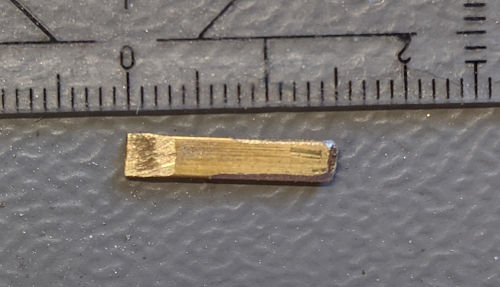
\includegraphics[width=7cm]{stift}};
\end{tikzpicture}
\caption{Kontaktstift} \label{fig:1}
\end{figure}

Die Stifte in die Kontaktfedern dr"ucken und danach die Platine aufsetzen. Ggf. Stifte etwas abrunden damit diese besser in die Platine passen. Stift 11 hat ggf. keine Feder, siehe \ref{sec:mod:erkennungta}. Falls Modifikation nicht durchgef"uhrt wird diesen Stift weglassen.

\begin{figure}[H]
\centering
\begin{tikzpicture}
     \node[anchor=south west,inner sep=0] at (0,0) {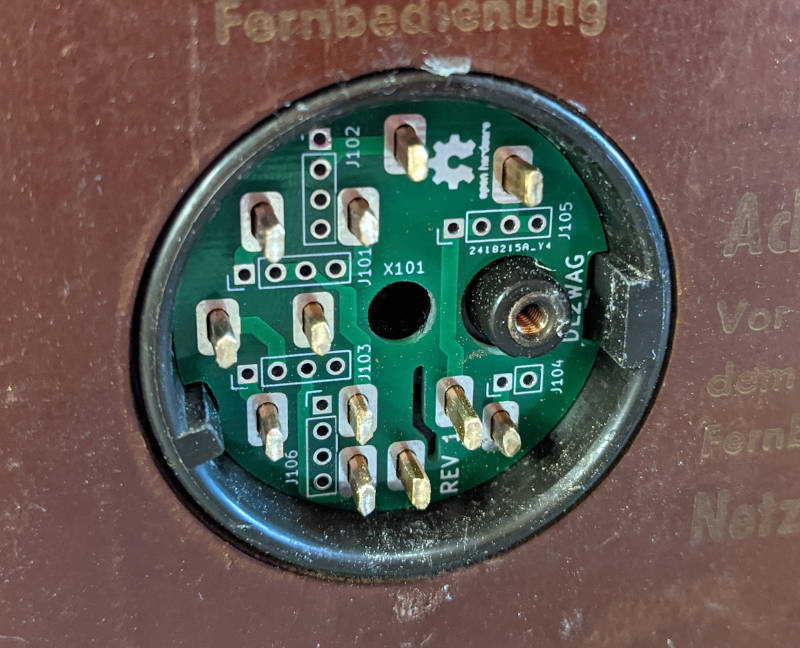
\includegraphics[width=10cm]{stecker-zusammen}};
\end{tikzpicture}
\caption{Stecker} \label{fig:1}
\end{figure}

Stifte in dieser Position verl"oten. Nur sehr kurz und mit hoher Leistung, sonst schmilzt der Kunststoff der Buchse! Mit Widerstandsmessger"at pr"ufen ob alle Stifte guten Kontakt zum jeweiligen Kontakt in der Buchse haben, ggf. nacharbeiten.


\begin{figure}[H]
\centering
\begin{tikzpicture}
     \node[anchor=south west,inner sep=0] at (0,0) {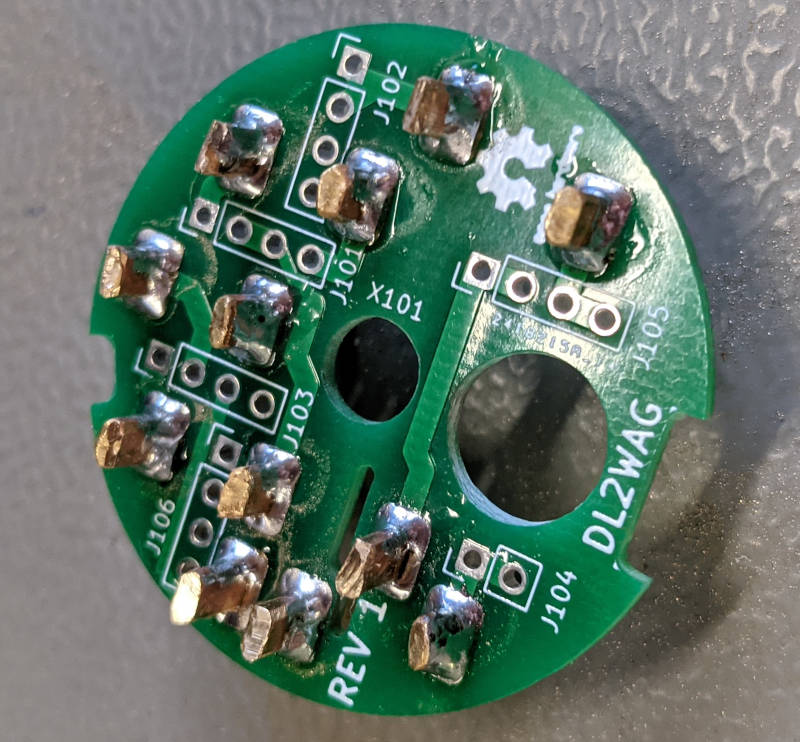
\includegraphics[width=.4\textwidth]{stecker-geloetet1}};
\end{tikzpicture}
\hspace{1cm} %no empty line!
\begin{tikzpicture}
     \node[anchor=south west,inner sep=0] at (0,0) {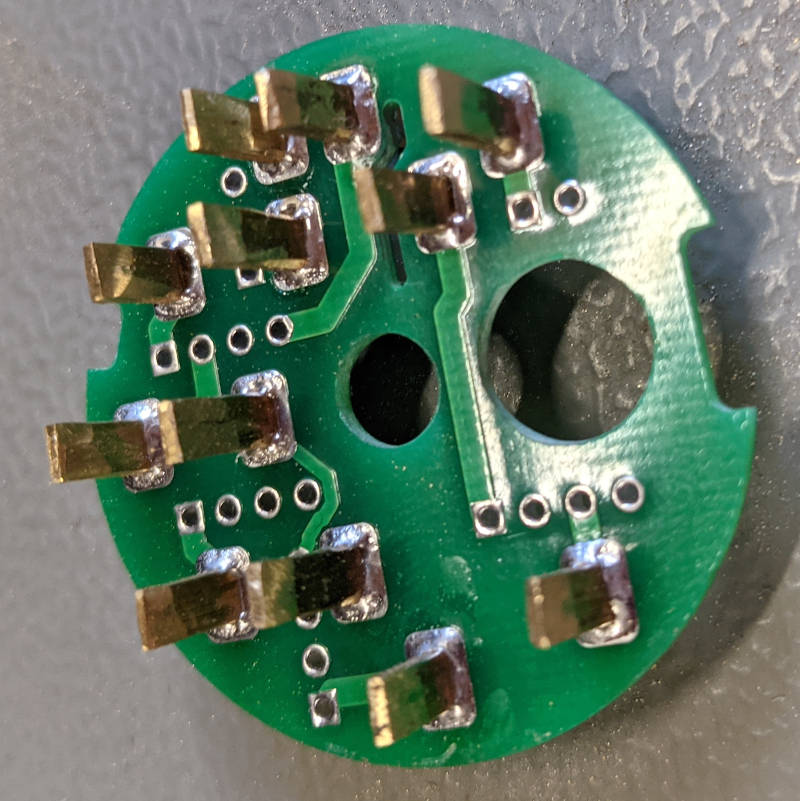
\includegraphics[width=.37\textwidth]{stecker-geloetet2}};
\end{tikzpicture}
\caption{Stecker gel"otet} \label{fig:1}
\end{figure}

Stiftleisten mit Platine verl"oten. Kunststoff so verschieben das die Stifte auf der Unterseite b"undig mit der Platine abschlie"sen (und der Stecker b"undig auf dem Kunststoff der Buchse aufsitzt). 

\begin{figure}[H]
\centering
\begin{tikzpicture}
     \node[anchor=south west,inner sep=0] at (0,0) {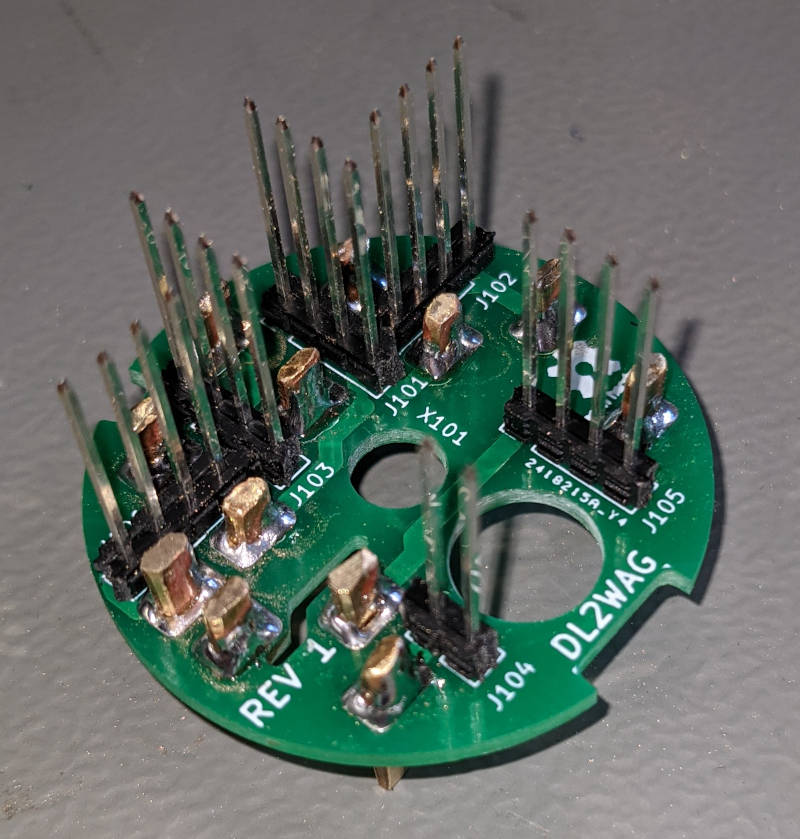
\includegraphics[width=.34\textwidth]{stecker-fertig1}};
\end{tikzpicture}
\hspace{1cm} %no empty line!
\begin{tikzpicture}
     \node[anchor=south west,inner sep=0] at (0,0) {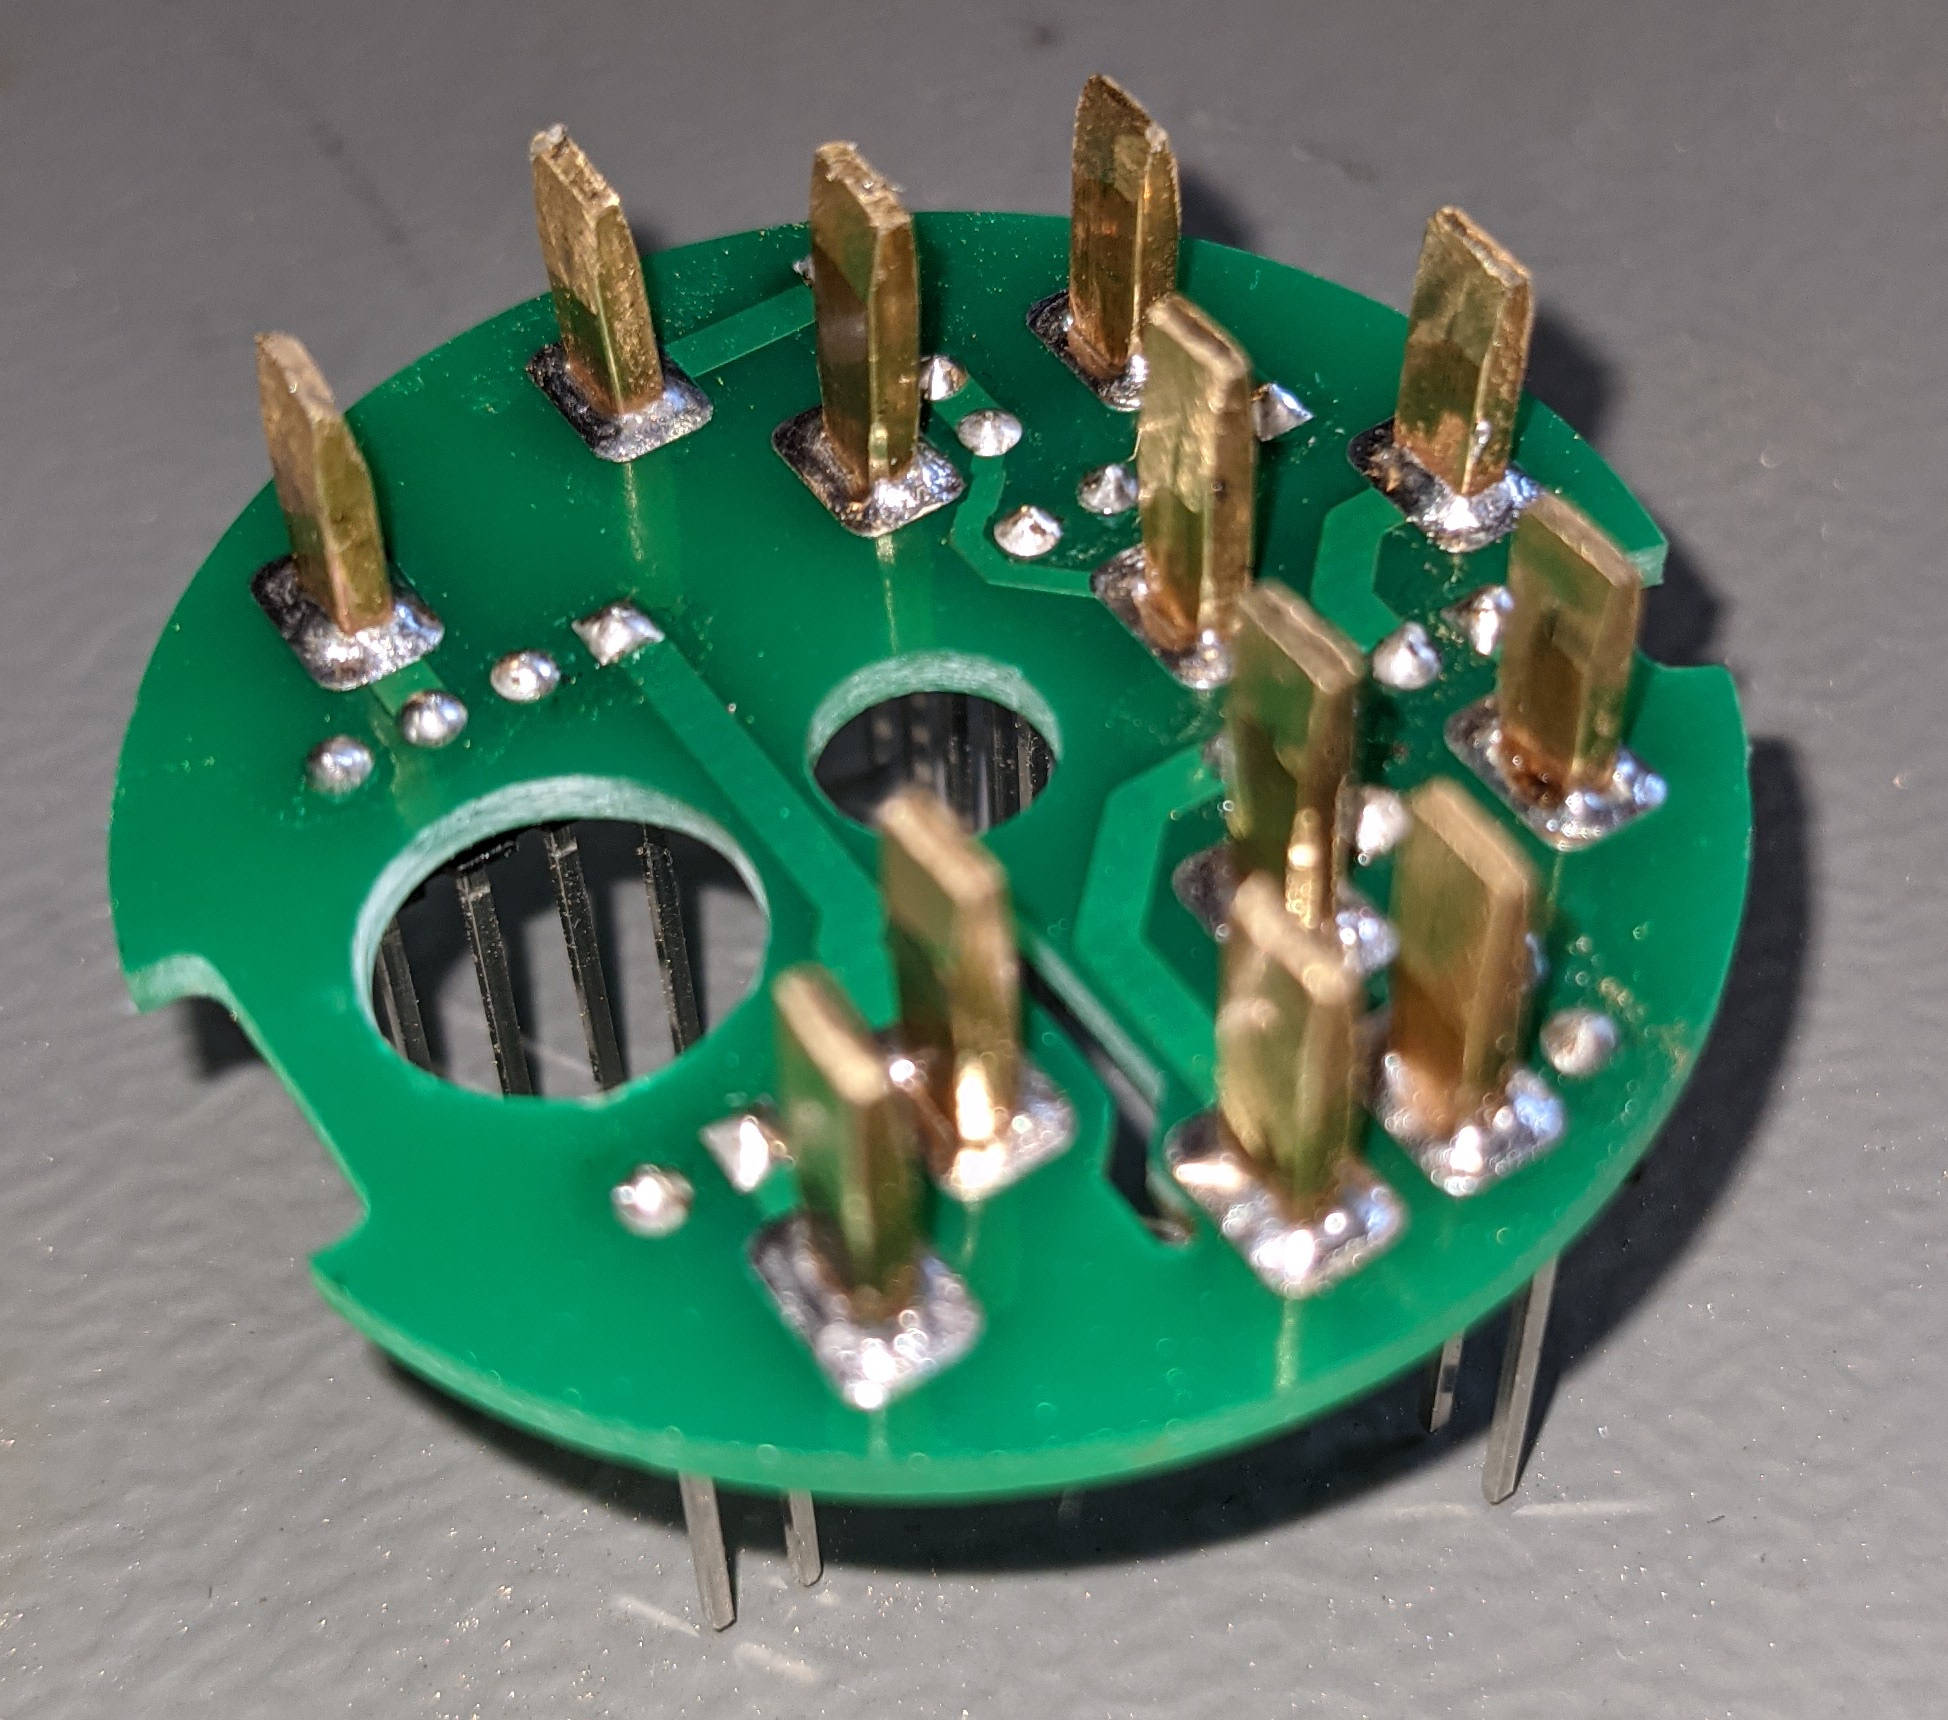
\includegraphics[width=.4\textwidth]{stecker-fertig2}};
\end{tikzpicture}
\caption{Stecker fertig} \label{fig:1}
\end{figure}

Holzstab auf ca. 4,5\,cm k"urzen und vorne mit Bleistifspitzer anspitzen. Hinten Loch f"ur Schraube bohren.

\begin{figure}[H]
\centering
\begin{tikzpicture}
     \node[anchor=south west,inner sep=0] at (0,0) {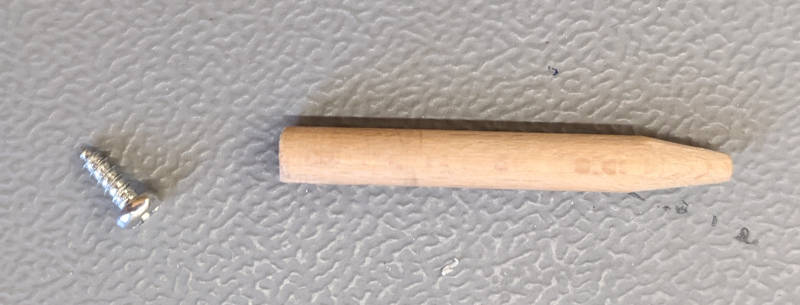
\includegraphics[width=6cm]{holzstab}};
\end{tikzpicture}
\caption{Zentrierstift} \label{fig:1}
\end{figure}

Der Stift muss durch das Loch in der Mitte des Steckers passen und wird auf die Steuerplatine aufgeschraubt.

\subsection{Steuerung} \label{sec:aufbau:steuerung}

Wir brauchen:
\begin{itemize}
\item Platine
\item Bauteile
\end{itemize}

Zuerst nicht ben"otigte herausstehende St"ucke der Platine abs"agen (USB und ggf. SD Karte). Dann kleine Bauteile aufl"oten (IC und ggf. SD Karte).

\begin{figure}[H]
\centering
\begin{tikzpicture}
     \node[anchor=south west,inner sep=0] at (0,0) {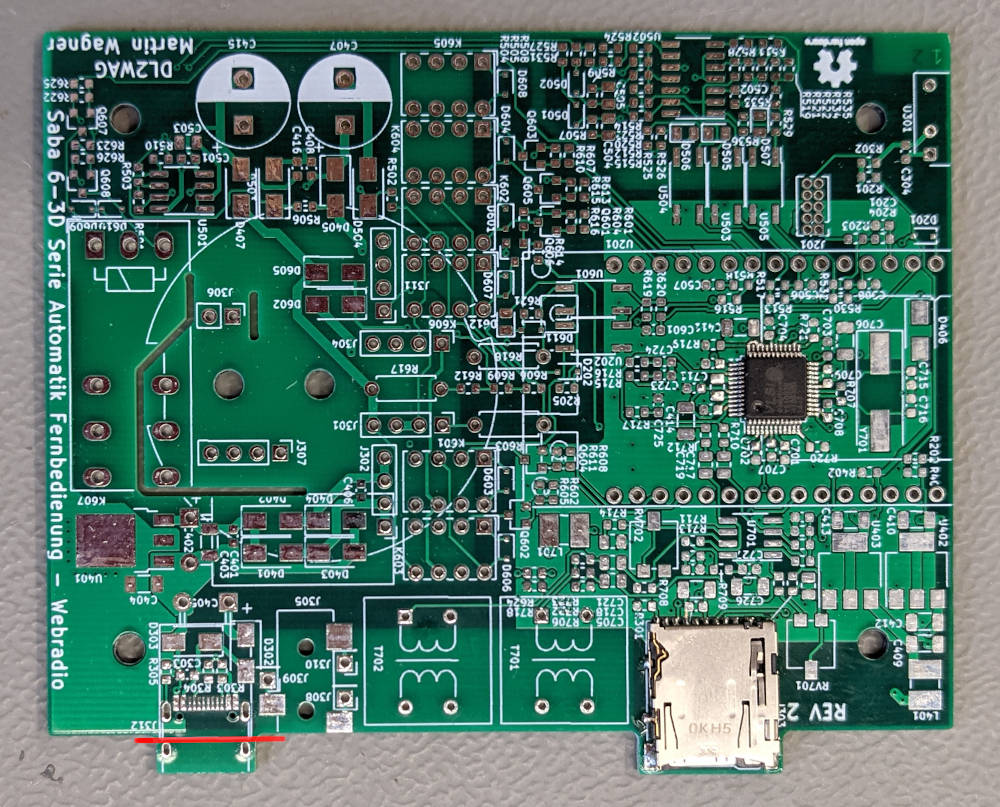
\includegraphics[width=.7\textwidth]{platine1}};
\end{tikzpicture}
\caption{Best"uckung kleine SMD Bauteile} \label{fig:1}
\end{figure}

Den Rest der Bauteile nacheinander best"ucken, beginnend um IC herum. "`NP"' Bauteile beachten (nicht best"ucken!). Kontakt 230\,V AC auf N1 oder N2 br"ucken, siehe \ref{sec:schaltung:steuern-radio}.

\begin{figure}[H]
\centering
\begin{tikzpicture}
     \node[anchor=south west,inner sep=0] at (0,0) {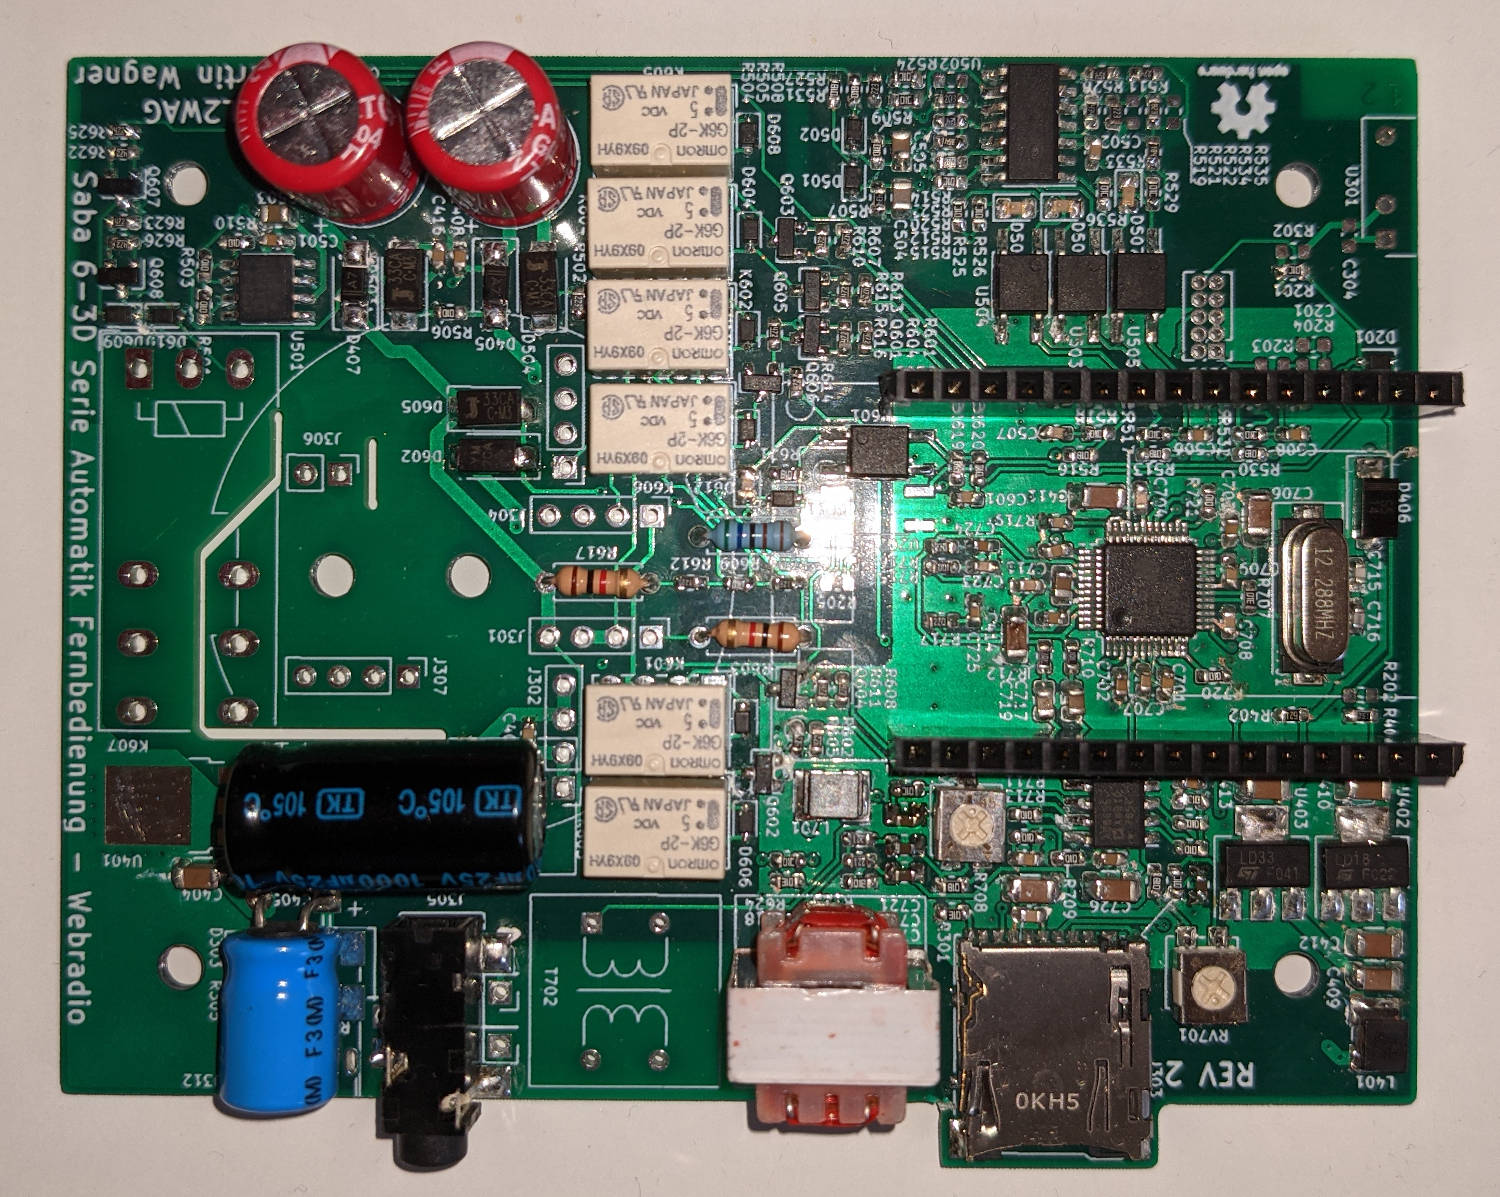
\includegraphics[width=.7\textwidth]{platine2}};
\end{tikzpicture}
\caption{Best"uckung fertig} \label{fig:1}
\end{figure}

\subsection{Montage} \label{sec:aufbau:montage}

Geh"ause f"ur Montage der Platine und Stecker vorbereiten. Der Mittelpunkt des Stecker Bohrlochs kann durch das Loch f"ur den Zentrierstift auf der Steuerplatine angezeichnet werden. Das Loch sollte so gro"s sein das der Stecker durchpasst (um die Baugruppe im sp"ateren Verlauf herausnehmen zu k"onnen).

\begin{figure}[H]
\centering
\begin{tikzpicture}
     \node[anchor=south west,inner sep=0] at (0,0) {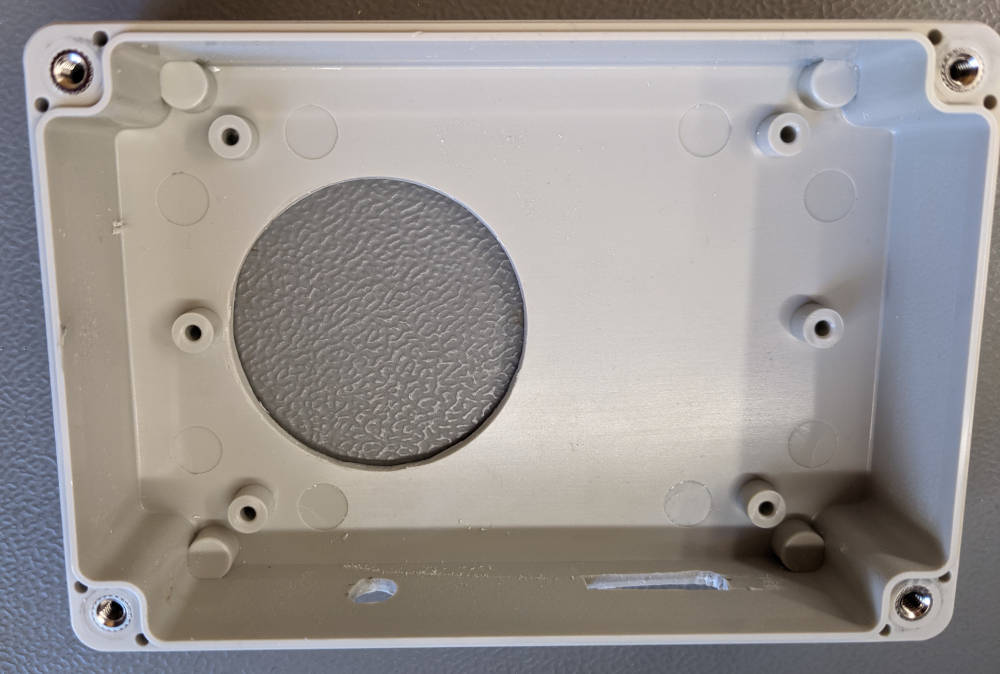
\includegraphics[width=8cm]{gehaeuse}};
\end{tikzpicture}
\caption{Geh"ause} \label{fig:1}
\end{figure}

Stecker in Buchse einstecken, Geh"ause mit montierter Steuerplatine b"undig aufsetzen. Stifte einrasten und verl"oten.

\begin{figure}[H]
\centering
\begin{tikzpicture}
     \node[anchor=south west,inner sep=0] at (0,0) {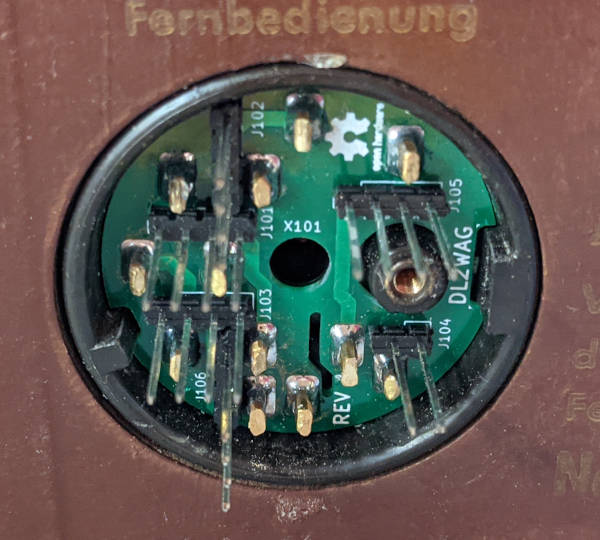
\includegraphics[width=.42\textwidth]{stecker-montieren}};
\end{tikzpicture}
\hspace{1cm} %no empty line!
\begin{tikzpicture}
     \node[anchor=south west,inner sep=0] at (0,0) {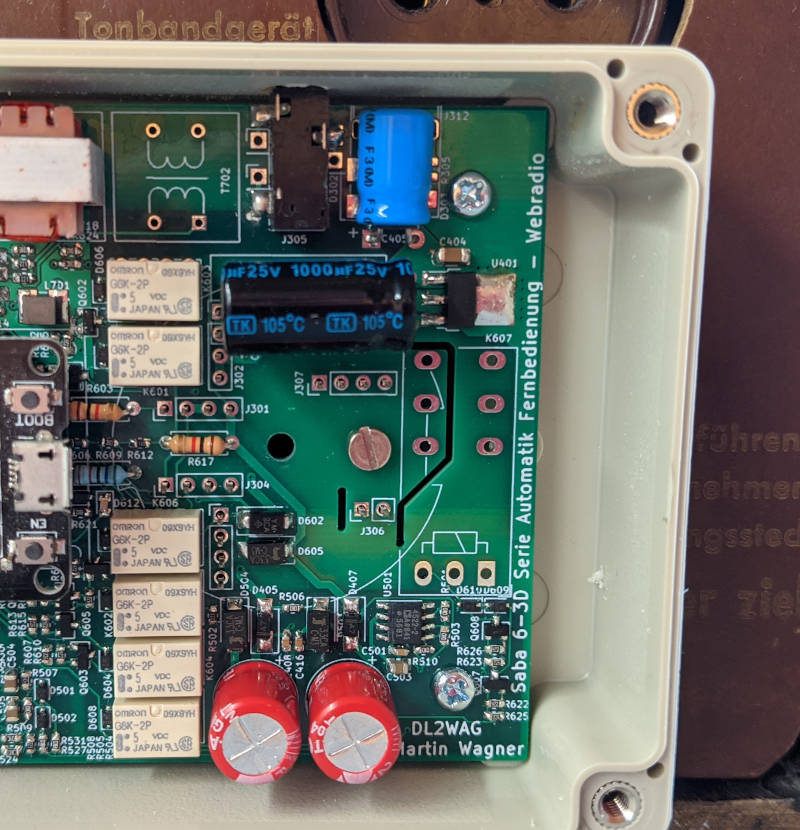
\includegraphics[width=.37\textwidth]{stecker-montieren2}};
\end{tikzpicture}
\caption{Stecker fertig} \label{fig:1}
\end{figure}

Zuletzt wird der Zentrierstift auf der Steuerplatine verschraubt.

\begin{figure}[H]
\centering
\begin{tikzpicture}
     \node[anchor=south west,inner sep=0] at (0,0) {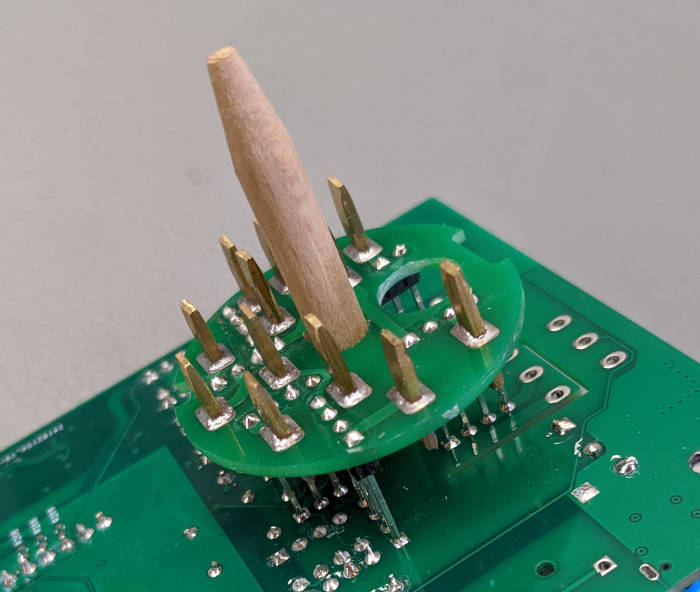
\includegraphics[width=6cm]{stift-montiert}};
\end{tikzpicture}
\caption{Zentrierstift im Stecker} \label{fig:1}
\end{figure}

Die gesamte Baugruppe kann jetzt nach dem Einstecken auf der Anschlussbuchse festgeschraubt werden. Vorsichtig, da Platine nicht auf der Buchse aufliegt.

\subsection{Inbetriebnahme / Test} \label{sec:aufbau:inbetriebnahme}

Die Steuerplatine sollte vor der Montage auf korrekte Funktion gepr"uft werden. Die einzelnen Schaltungsteile werden unabh"angig voneinander betrachtet.

\textbf{Spannungsversorgung Mikrocontroller}

Die Versorgung wird aus der Heizspannung 6,3\,V durch Vollweggleichrichtung + darauffolgend 5\,V Linearregler gewonnen. Folgende Spannungen stehen zur Verf"ugung\footnote{Siehe Schaltplan Seite 3}:
\begin{itemize}
\item ca. 8\,V
\item 5,0\,V
\item 3,3\,V Digital (werden vom ESP32 ausgegeben)
\item 1,8\,V Digital
\item 3,3\,V Analog
\end{itemize}

\textbf{Spannungsversorgung Suchlauf}

Die Versorgung wird aus der 2x15\,V Spannungsversorgung f"ur den Suchlauf durch Einweggleichrichtung gewonnen. Folgende Spannungen stehen zur Verf"ugung:
\begin{itemize}
\item ca. +/- 20\,V
\end{itemize}

\begin{figure}[H]
\centering
\begin{tikzpicture}
     \node[anchor=south west,inner sep=0] at (0,0) {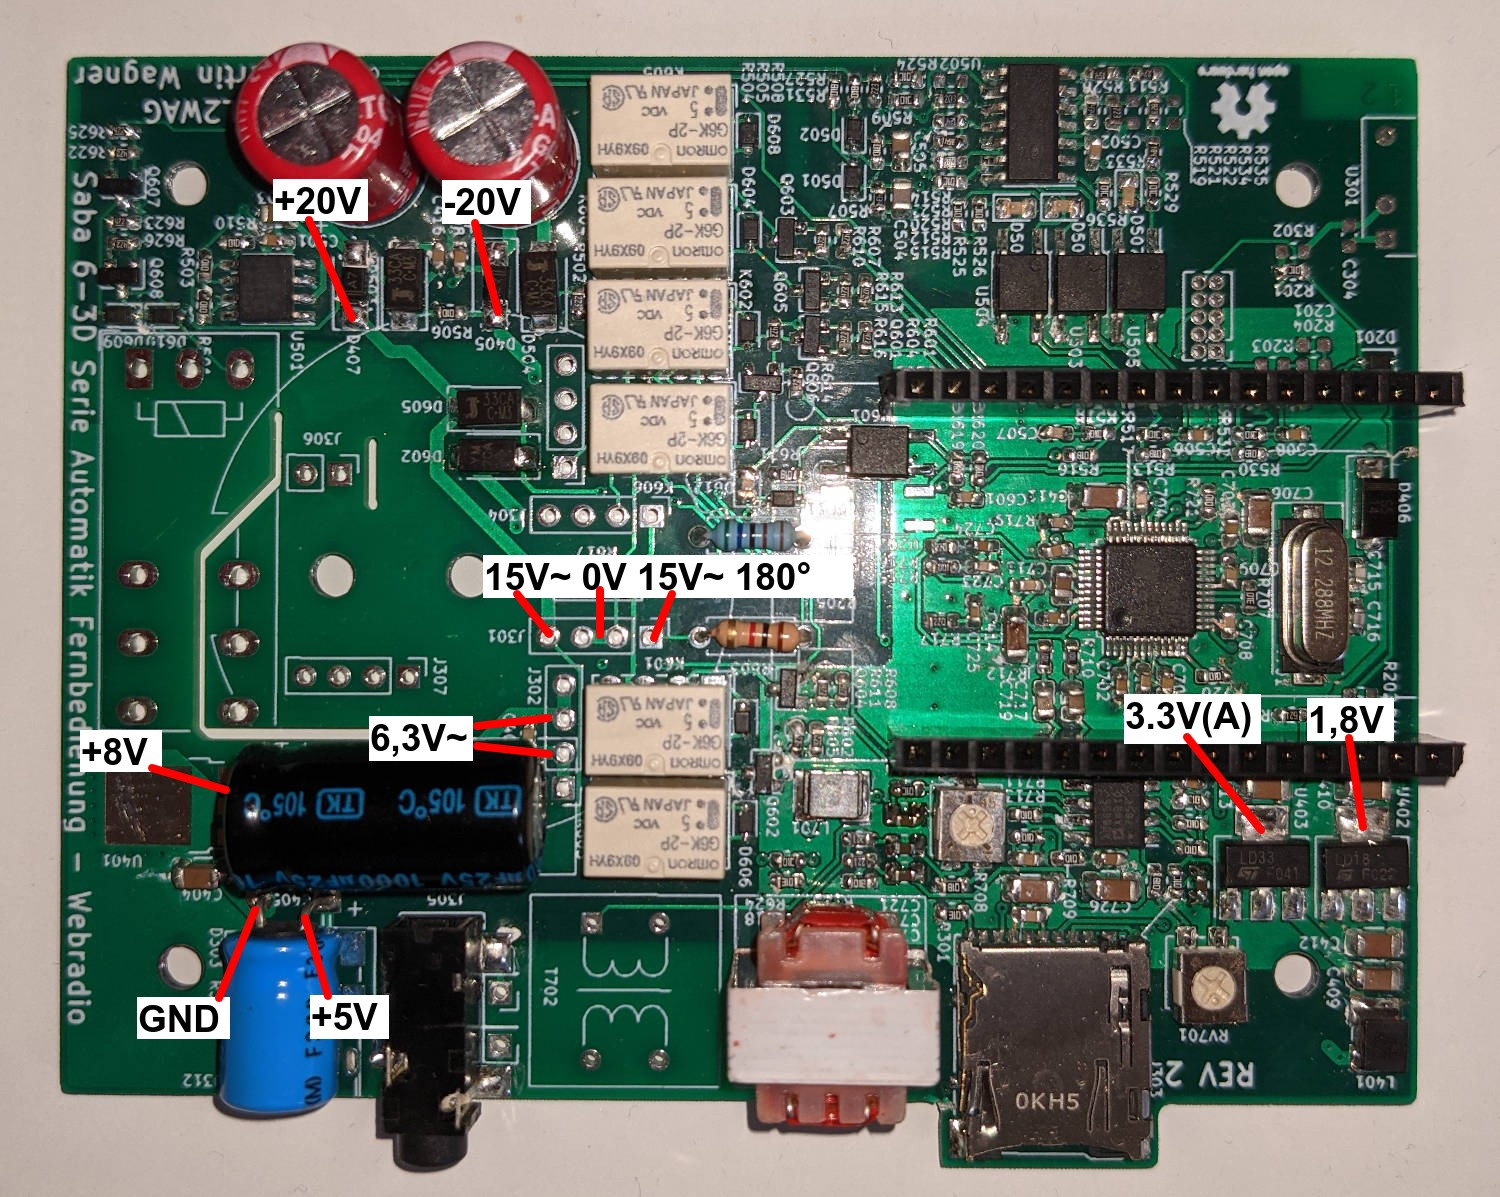
\includegraphics[width=.7\textwidth]{platine3}};
\end{tikzpicture}
\caption{DC Spannungen Messpunkte} \label{fig:1}
\end{figure}

\textbf{Suchlauf Operationsverst"arker / Komparatoren}

Versorgungsspannung 2x15\,V AC -- +/-20\,V. Die Comparatoren sind auf eine Versorgungsspannung von 22\,V berechnet. Da in der Schaltung Spannungsverh"altnisse verglichen werden sind die berechneten Schaltschwellen nur bei dieser Spannung g"ultig. Bei anderen Versorgungsspannungen verschieben sich die Schaltpunkte proportional zur Versorgungsspannung.

Alle Messungen mit Bezug auf die Mittelanzapfung der 15\,V Wicklung, nicht Masse des Radios! Beim Messen aufpassen das nicht versehentlich die verschiedenen Massepotentiale verbunden werden! Suchlauftaste am Ger"at bet"atigen (Suchlauf aus) oder Suchlaufschaltung auf Breadboard nachbauen.

\begin{figure}[H]
\centering
\begin{tikzpicture}
     \node[anchor=south west,inner sep=0] at (0,0) {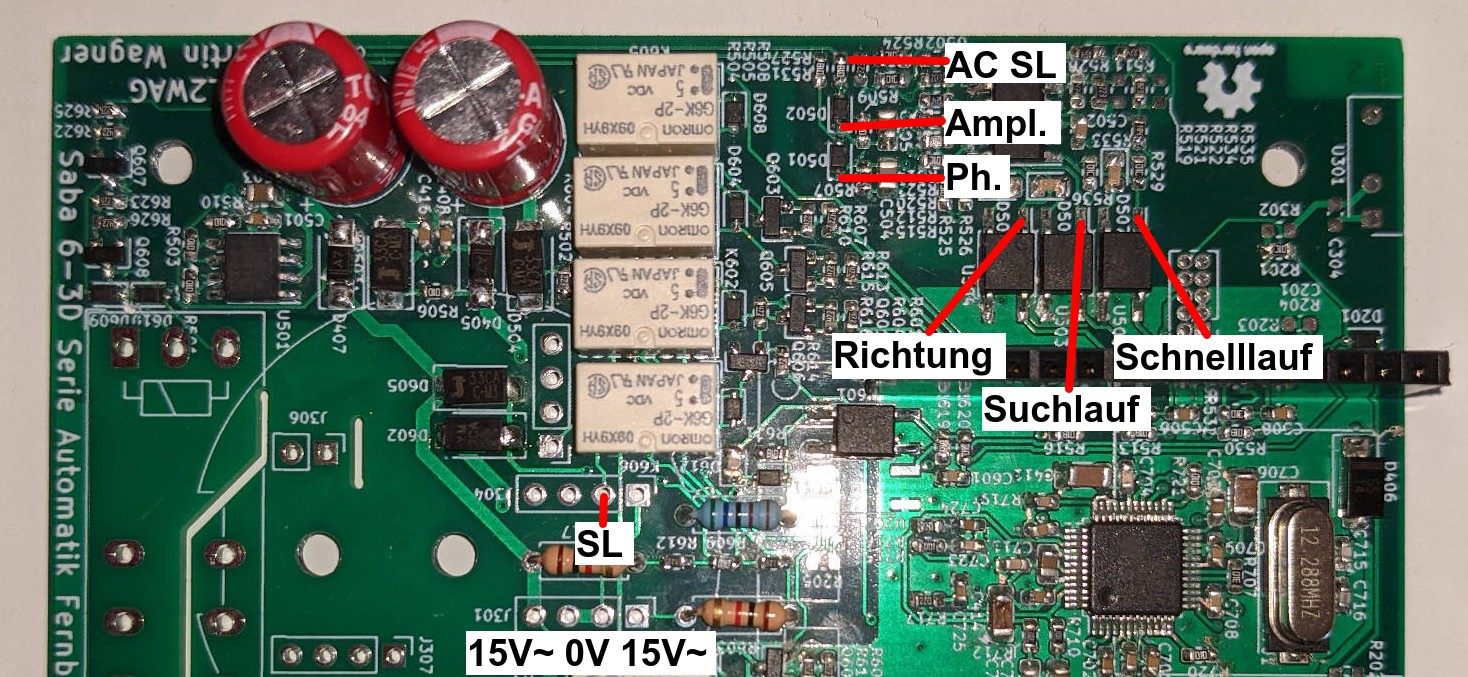
\includegraphics[width=\textwidth]{platine4}};
\end{tikzpicture}
\caption{AC Messpunkte} \label{fig:1}
\end{figure}

\begin{figure}[H]
\centering
\begin{tikzpicture}
     \node[anchor=south west,inner sep=0] at (0,0) {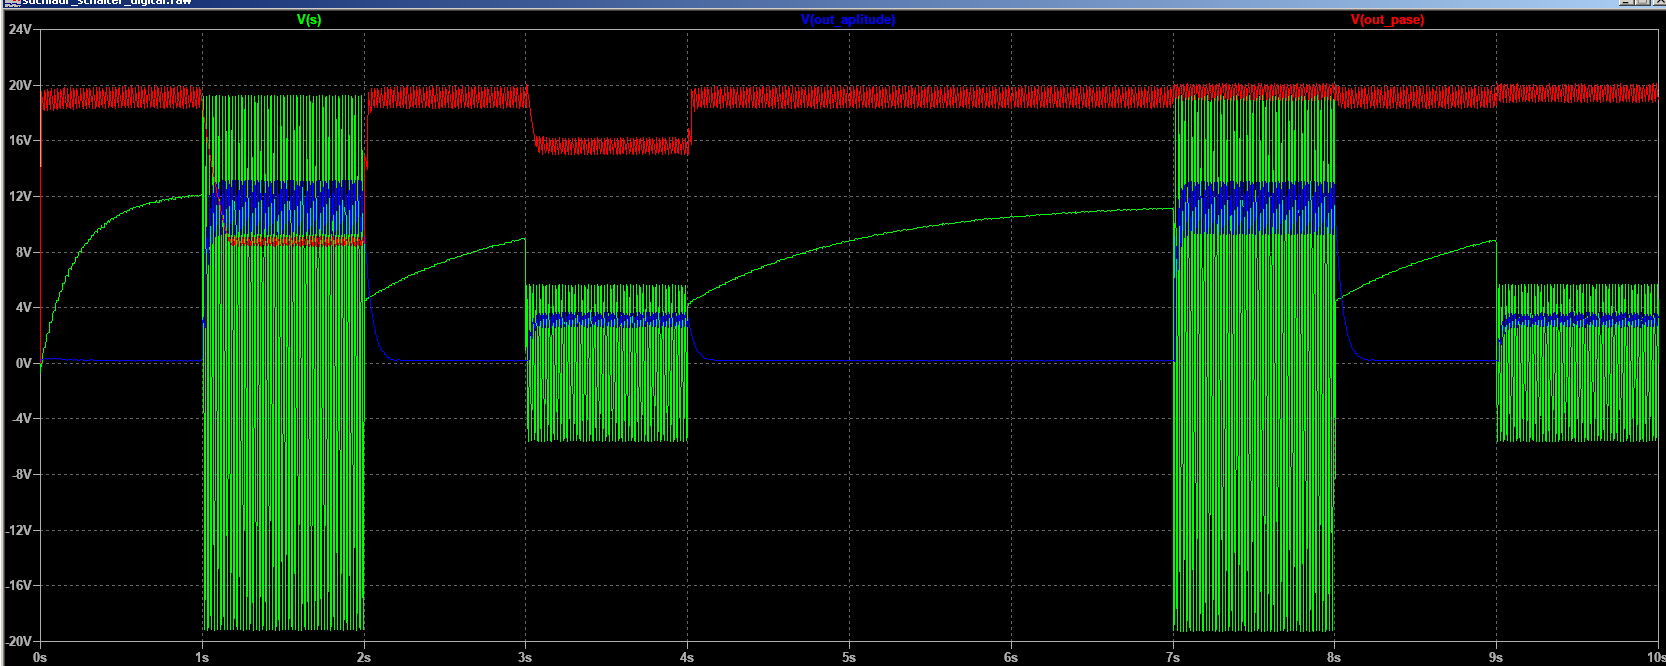
\includegraphics[width=\textwidth]{messen2.png}};
\end{tikzpicture}
\caption{Spannungen in Simulation} \label{fig:1}
\end{figure}

\textbf{Messungen Signal Laufrichtung}

\begin{figure}[H]
\centering
\begin{tikzpicture}
     \node[anchor=south west,inner sep=0] at (0,0) {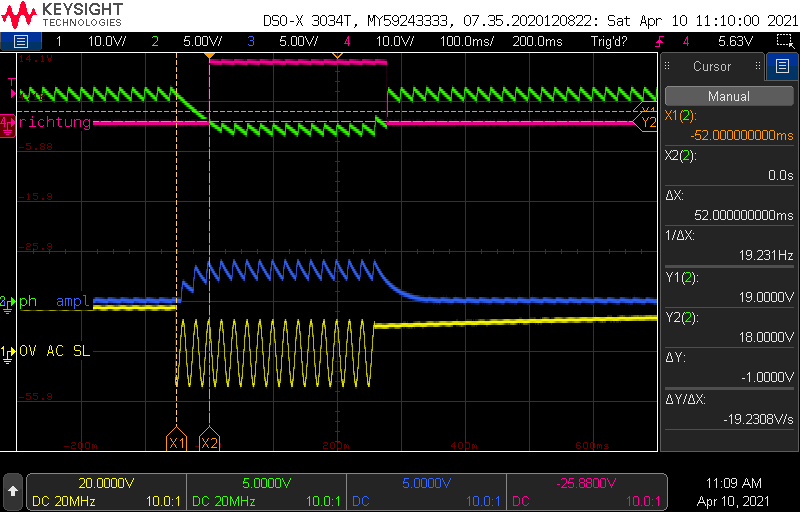
\includegraphics[width=\tscopesize]{image27346.png}};
\end{tikzpicture}
\caption{Laufrichtung 1, suchen} \label{fig:1}
\end{figure}

\begin{figure}[H]
\centering
\begin{tikzpicture}
     \node[anchor=south west,inner sep=0] at (0,0) {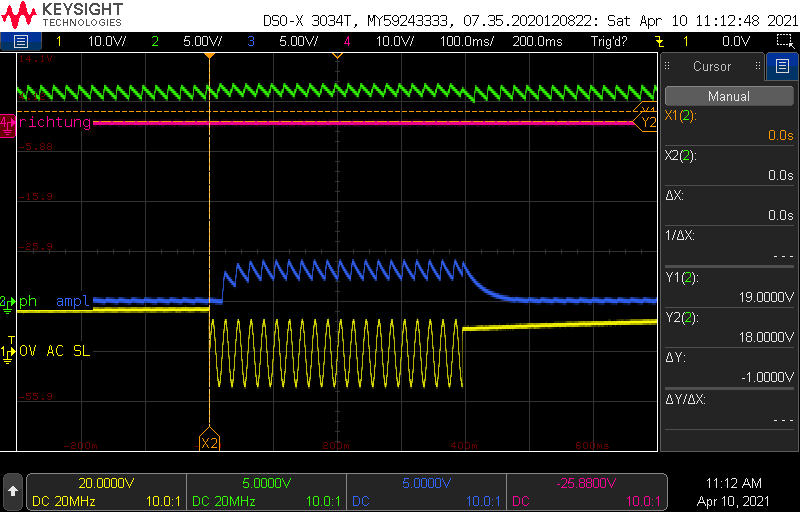
\includegraphics[width=\tscopesize]{image17823.png}};
\end{tikzpicture}
\caption{Laufrichtung 2, suchen} \label{fig:1}
\end{figure}

\begin{figure}[H]
\centering
\begin{tikzpicture}
     \node[anchor=south west,inner sep=0] at (0,0) {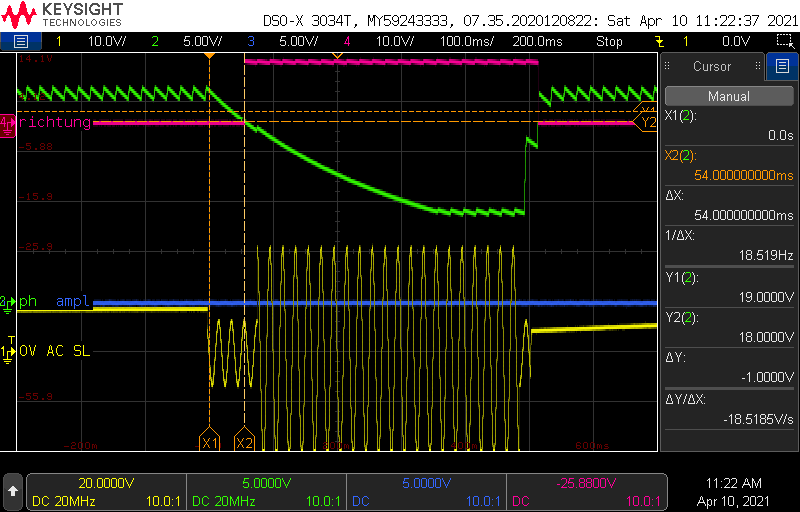
\includegraphics[width=\tscopesize]{image9355.png}};
\end{tikzpicture}
\caption{Laufrichtung 1, schnell} \label{fig:1}
\end{figure}

\begin{figure}[H]
\centering
\begin{tikzpicture}
     \node[anchor=south west,inner sep=0] at (0,0) {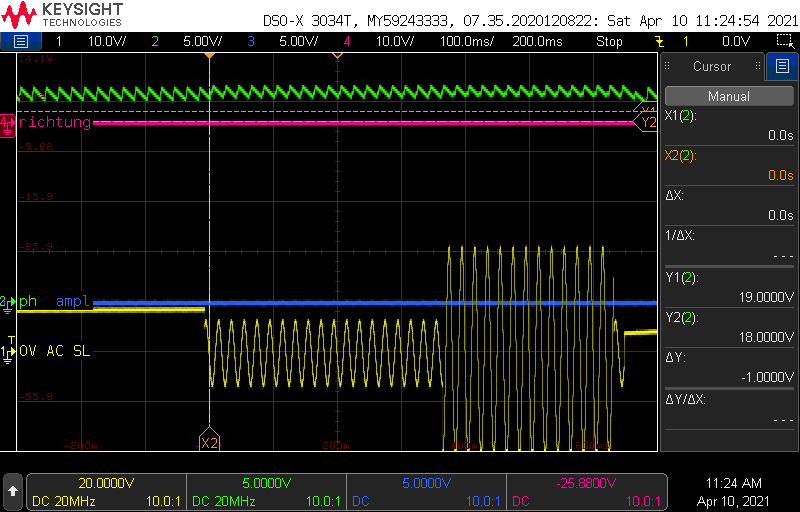
\includegraphics[width=\tscopesize]{image29704.png}};
\end{tikzpicture}
\caption{Laufrichtung 2, schnell} \label{fig:1}
\end{figure}

Die Laufrichtung muss korrekt erkannt werden. Die Verz"ogerung muss im Bereich bis max. ca 50\,ms sein. Beim Schnelllauf wird zuerst der Kontakt f"ur den Suchlauf geschlossen, bereits dieser f"uhrt zur Erkennung.

\textbf{Signal Laufrichtung im Bereich der zul"assigen Versorgungsspannung}

Die Versorgungsspannung f"ur den Schaltungsteil ist nicht stabilisiert und schwankt daher in Abh"angikeit der Netzspannung.

Sweep Versorgungsspannung +/- 10\,V ... 18\,V AC. 

\begin{figure}[H]
\centering
\begin{tikzpicture}
     \node[anchor=south west,inner sep=0] at (0,0) {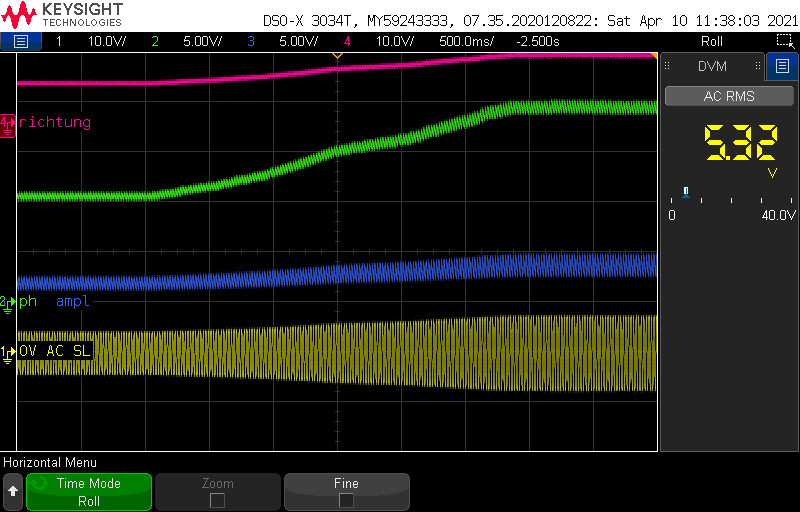
\includegraphics[width=\tscopesize]{image22258.png}};
\end{tikzpicture}
\caption{Laufrichtung 1, suchen} \label{fig:1}
\end{figure}

Das digitale Signal steht im gesamten Versorgungsspannungsbereich korrekt an. 

\textbf{Messungen Signal Schnelllauf}

\begin{figure}[H]
\centering
\begin{tikzpicture}
     \node[anchor=south west,inner sep=0] at (0,0) {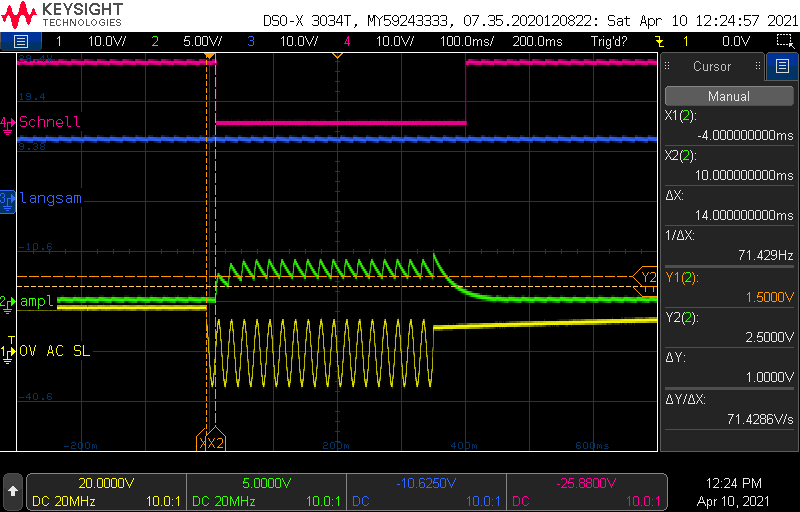
\includegraphics[width=\tscopesize]{image24190.png}};
\end{tikzpicture}
\caption{suchen} \label{fig:1}
\end{figure}

\begin{figure}[H]
\centering
\begin{tikzpicture}
     \node[anchor=south west,inner sep=0] at (0,0) {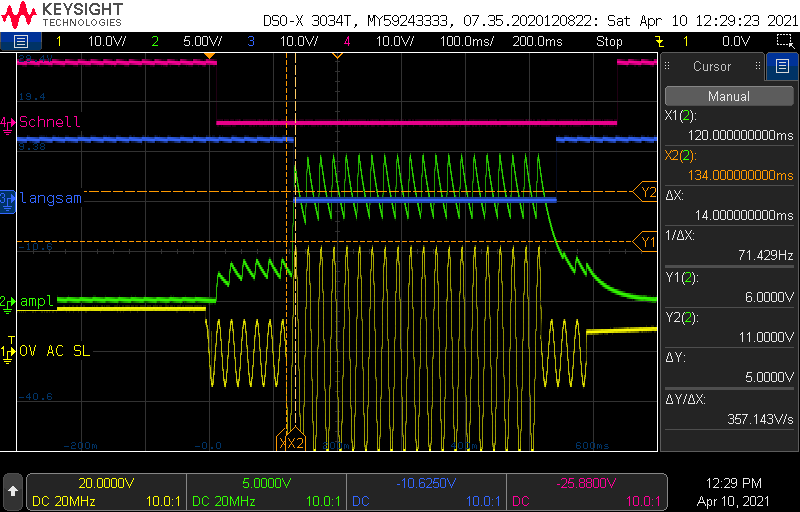
\includegraphics[width=\tscopesize]{image9293.png}};
\end{tikzpicture}
\caption{schnelllauf} \label{fig:1}
\end{figure}

Der Schnelllauf muss korrekt erkannt werden. Die Verz"ogerung muss im Bereich bis max. ca 50\,ms sein. 

\textbf{Signal Schnelllauf im Bereich der zul"assigen Versorgungsspannung}

Sweep Versorgungsspannung +/- 10\,V ... 18\,V AC. 

\begin{figure}[H]
\centering
\begin{tikzpicture}
     \node[anchor=south west,inner sep=0] at (0,0) {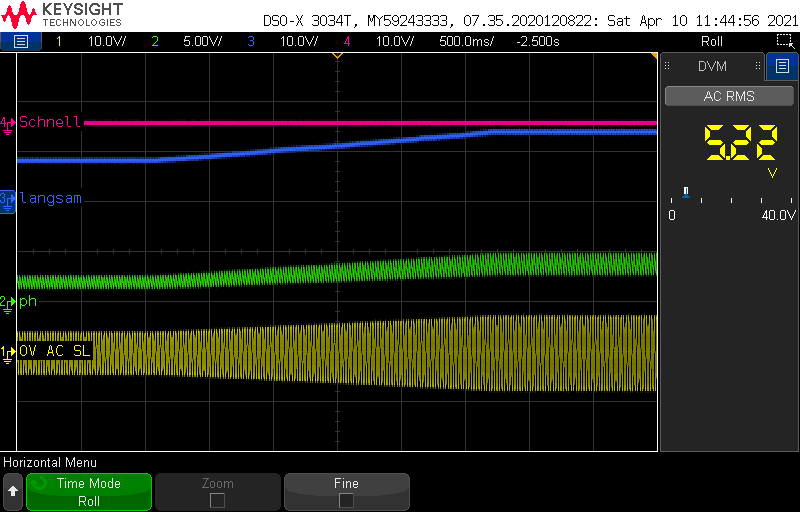
\includegraphics[width=\tscopesize]{image22512.png}};
\end{tikzpicture}
\caption{suchen} \label{fig:1}
\end{figure}

\begin{figure}[H]
\centering
\begin{tikzpicture}
     \node[anchor=south west,inner sep=0] at (0,0) {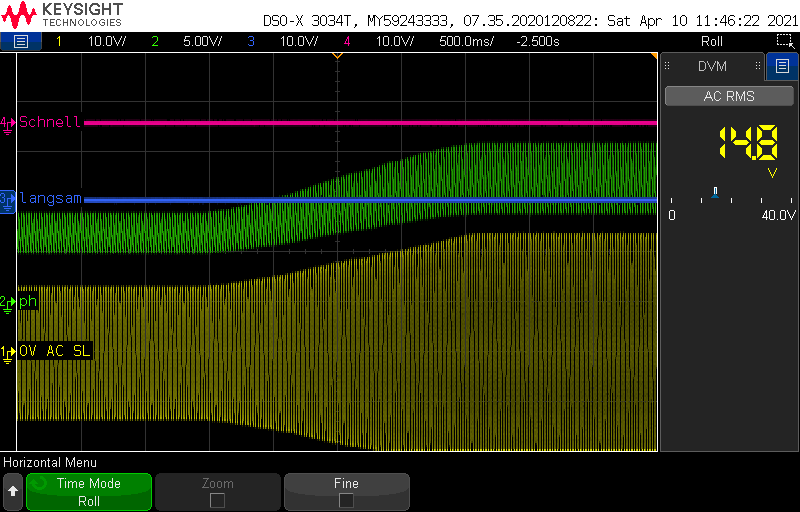
\includegraphics[width=\tscopesize]{image9576.png}};
\end{tikzpicture}
\caption{schnelllauf} \label{fig:1}
\end{figure}

Das digitale Signal steht im gesamten Versorgungsspannungsbereich korrekt an. 

\textbf{Haltespule}

Die Funktion der "`Haltespule"' kann durch das Anlegen von ca. 35\,V AC getestet werden.

\begin{figure}[H]
\centering
\begin{tikzpicture}
     \node[anchor=south west,inner sep=0] at (0,0) {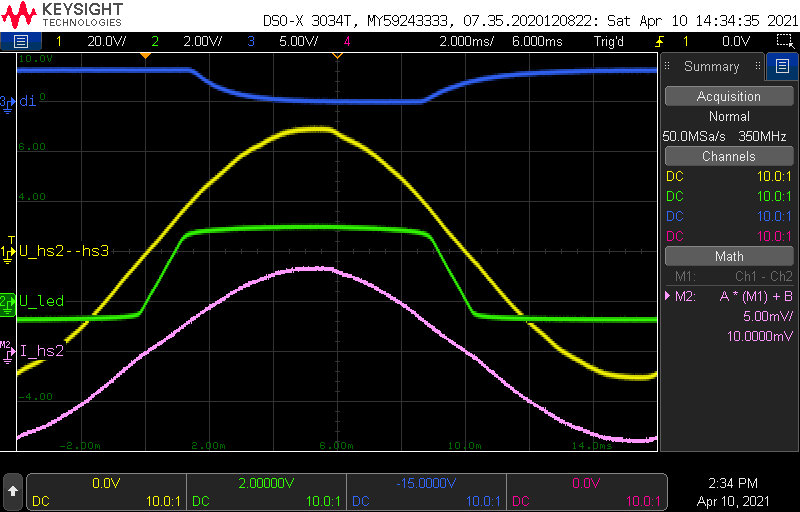
\includegraphics[width=\tscopesize]{image31192.png}};
\end{tikzpicture}
\caption{Haltespule} \label{fig:1}
\end{figure}

Der digitale Eingang muss bei ca. 30\,V / 5\,mA umschalten.

\textbf{Digitale Signale Mikrocontroller}

Die Signale am ESP32 k"onnen auf zwei M"oglichkeiten getestet werden:
\begin{itemize}
\item Spannungsquelle (Relais) + Multimeter (Eing"ange) anstelle des ESP32 an der Stiftleiste anschlie"sen
\item ESP32 + Arduino Testsoftware\footnote{Verzeichnis "`software/test"', aufspielen wie in \ref{sec:aufbau:programmierung} "`Arduino"'}
\end{itemize}

Signale nacheinander anlegen, es muss der zugeh"orige Eingang umschalten bzw. das zugeh"orige Relais schalten.

\textbf{Webradio / Audio Mikrocontroller}

Nicht vorab m"oglich. Nachdem ESP32 programmiert ist kann das Webradio wie in \ref{sec:bedienung}. beschrieben benutzt werden, an die Klinkenbuchse kann ein Kopfh"orer, PC Lautsperecher o."a. angeschlossen werden.

\subsection{Programmierung ESP32} \label{sec:aufbau:programmierung}

Der ESP32 Controller kann sowohl auserhalb wie auch in der Schaltung programmiert werden. Im letzten Fall ist \textbf{\color{red} penibelst} darauf zu achten dass das Ger"atechassis nicht geerdet ist. Grund: Der Schaltungs GND entspricht nicht dem Radio GND (Chassis), siehe Steuerplatine\footnote{Seite 4, Spannungsversorgung 5\,V}. Werden beide "uber das USB Programmierkabel verbunden entsteht ein Kurzschluss.

\textbf{M"oglichkeit 1: Kommandozeile, Python -- esptool.py}

Funktionierende Pythoninstallation mit \emph{pip} wird vorrausgesetzt. Sollte dann mit allen Betriebssystemen etwa gleich funktionieren. Normalerweise erkennt \emph{esptool.py} automatisch die richtige Schnittstelle, falls nicht kann man nachhelfen mit \emph{-{}-port /dev/ttyUSBx} (Linux) oder \emph{-{}-port COMx} (Windows).

Vorcompilierte Binaries sind im Verzeichnis "`software/bin"' abgelegt.

\begin{itemize}
\item \texttt{\$ pip install esptool}
\item ESP Board mit PC USB verbinden
\item Verbindung testen und ggf. vorhandene Altlasten entfernen:\\
		\texttt{\$ esptool.py erase\_flash}
\item Bootloader und Firmware programmieren:\\
		\texttt{\$ esptool.py --chip esp32  --baud 921600 --before default\_reset --after hard\_reset write\_flash -z --flash\_mode dio --flash\_freq 80m --flash\_size detect 0xe000 boot\_app0.bin 0x1000 bootloader\_dio\_80m.bin 0x10000 \\ESP32\_Radio.bin 0x8000 ESP32\_Radio.partitions.bin}
\end{itemize}

Ein Firmwareupdate kann einfach durch erneutes Aufrufen des Programmierkomandos durchgef"uhrt werden. Die Einstellungen bleiben dann erhalten.

\emph{\href{https://docs.espressif.com/projects/esptool/en/latest/esp32s3/esptool/index.html}{esptool.py Dokumentation}}. Die Kommandozeilenbefehle werden beim Compilieren / Hochladen durch die Arduino Umgebung ausgegeben.

\textbf{M"oglichkeit 2: Kommandozeile, PlatformIO}

In 2024 einfachste M"oglichkeit zu compilieren. Auch hier wird eine funktionierende Pythoninstallation vorrausgesetzt.

\begin{itemize}
\item Installieren nach \url{https://docs.platformio.org/en/latest/core/installation/methods/index.html}. Inklusive "`Install Shell Commands"'.
\item Sourcecode von der in \ref{sec:sabawebradio}. "`Software"' angegebenen URL herunterladen.
\item Ins Download Verzeichnis wechseln
\item Projekt vorbereiten:\\
		\texttt{\$ pio project init --board esp32doit-devkit-v1}
\item Projekt compilieren und "ubertragen:\\
		\texttt{\$ pio run upload}
\end{itemize}

\textbf{M"oglichkeit 3: Eclipse IDE}

Falls man ernsthaft etwas am Sourcecode "andern will empfehle ich ausdr"ucklich eine richtige IDE zu verwenden (Eclipse, VS-Code, ...).

\begin{itemize}
\item Wie "`PlatformIO".
\item Projekt vorbereiten:\\
		\texttt{\$ pio project init  --ide eclipse --board esp32doit-devkit-v1}
\item In Eclipse importieren nach \url{https://docs.platformio.org/en/latest/integration/ide/eclipse.html}. Verh"alt sich wie ein normales Eclipse Projekt.
\end{itemize}


\section{Bedienung} \label{sec:bedienung}

Webradio hinten auf Anschlusstecker aufstecken und mit Schraube festschrauben. Geh"ausedeckel aufschrauben. Audiokabel mit TA Buchsen verbinden.

\subsection{W-Lan Anmeldung} \label{sec:bedienung:wlan}

Bei der ersten Inbetriebnahme, oder falls das eingestellte W-Lan nicht erreichbar ist, "offnet der ESP32 ein offenes W-Lan Netz. Darin einloggen, IP \emph{192.168.4.1} im Webbrowser "offnen.

\begin{figure}[H]
\centering
\begin{tikzpicture}
     \node[anchor=south west,inner sep=0] at (0,0) {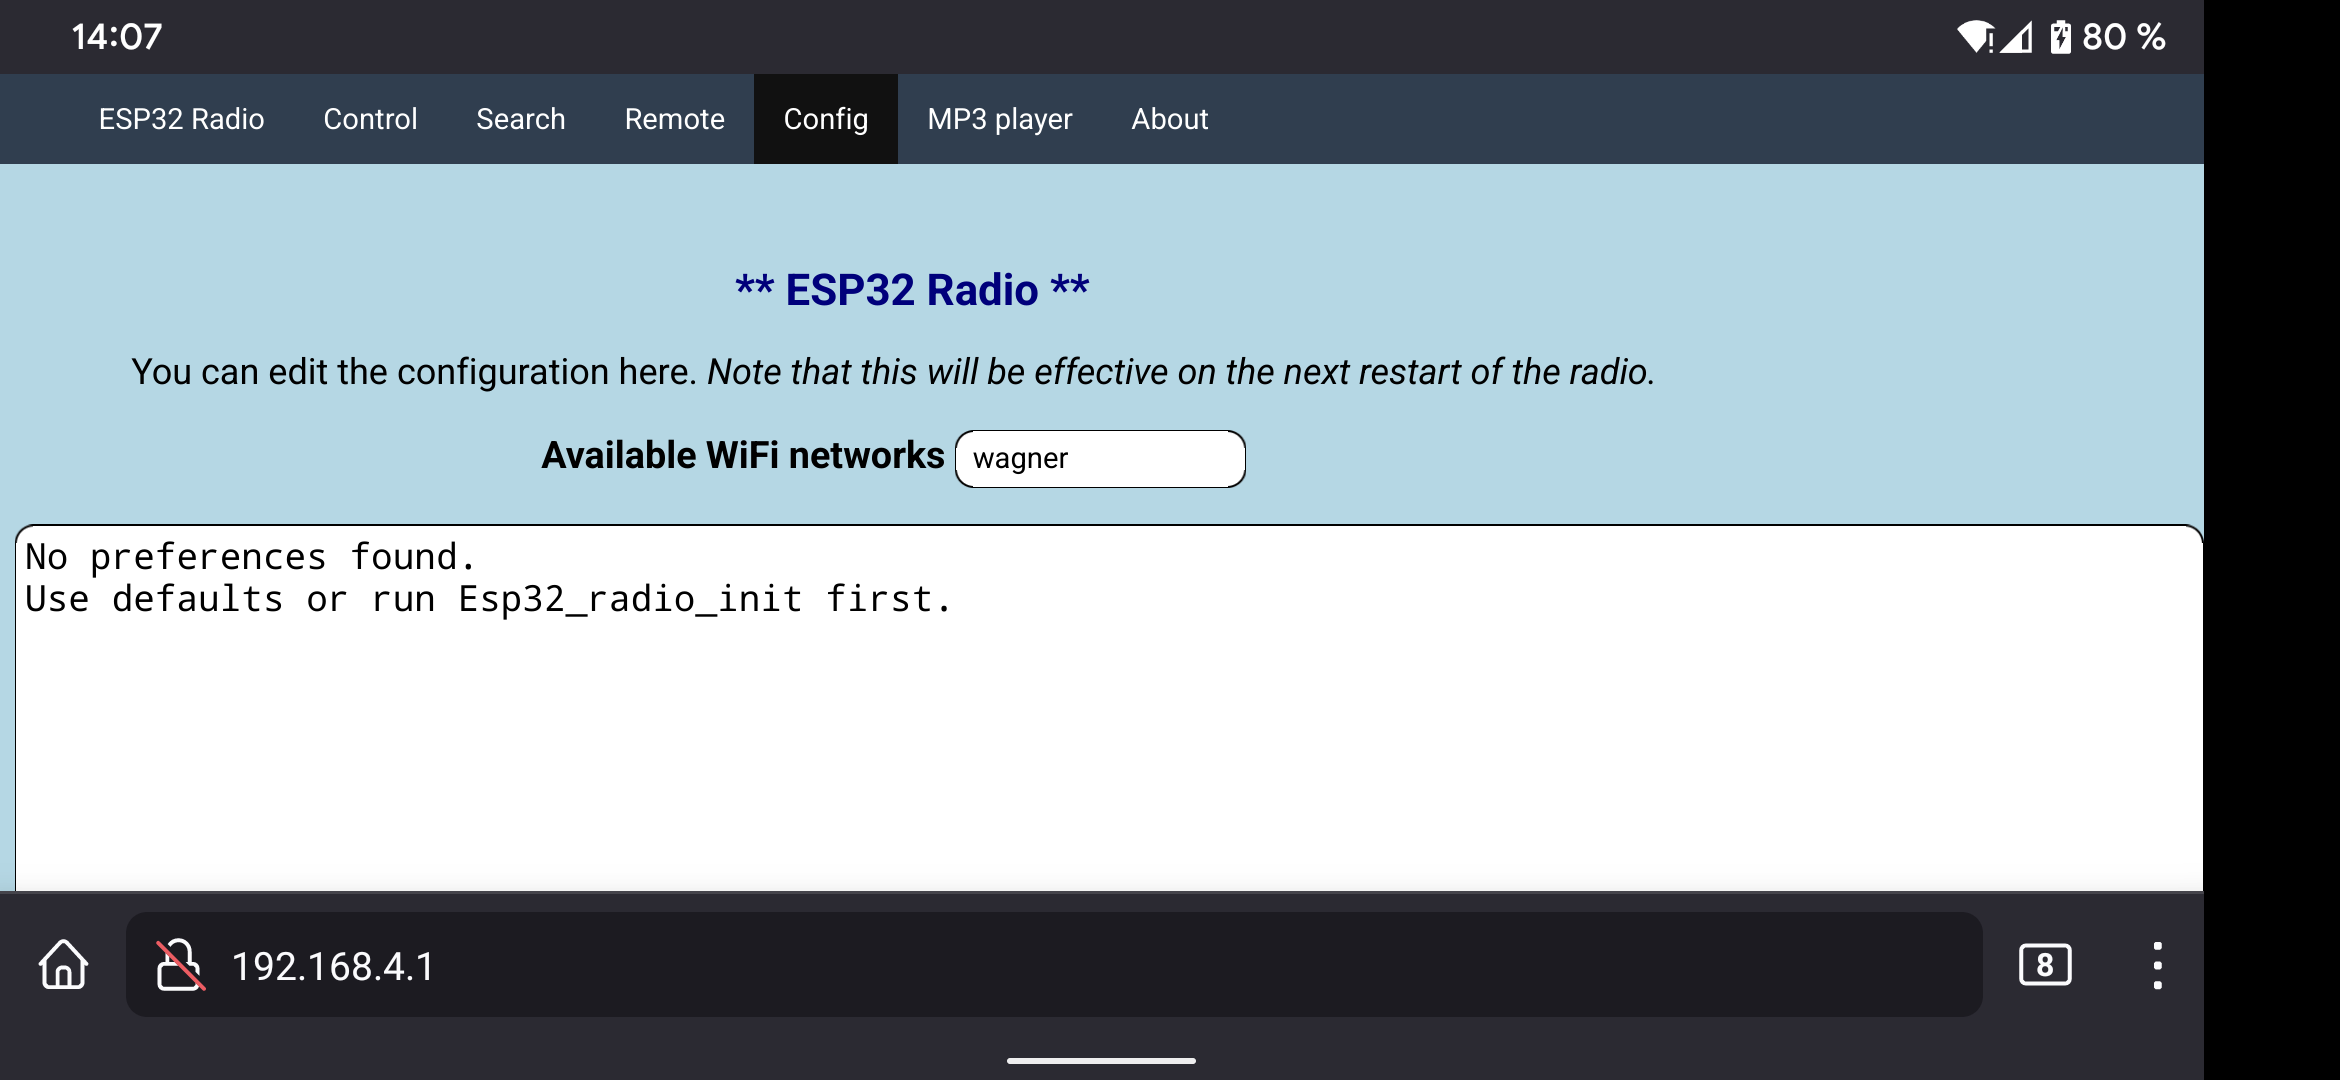
\includegraphics[width=\textwidth]{wlan1}};
\end{tikzpicture}
\caption{Startseite} \label{fig:1}
\end{figure}

Bis zum Ende scrollen, Knopf "`Default"' dr"ucken.

\begin{figure}[H]
\centering
\begin{tikzpicture}
     \node[anchor=south west,inner sep=0] at (0,0) {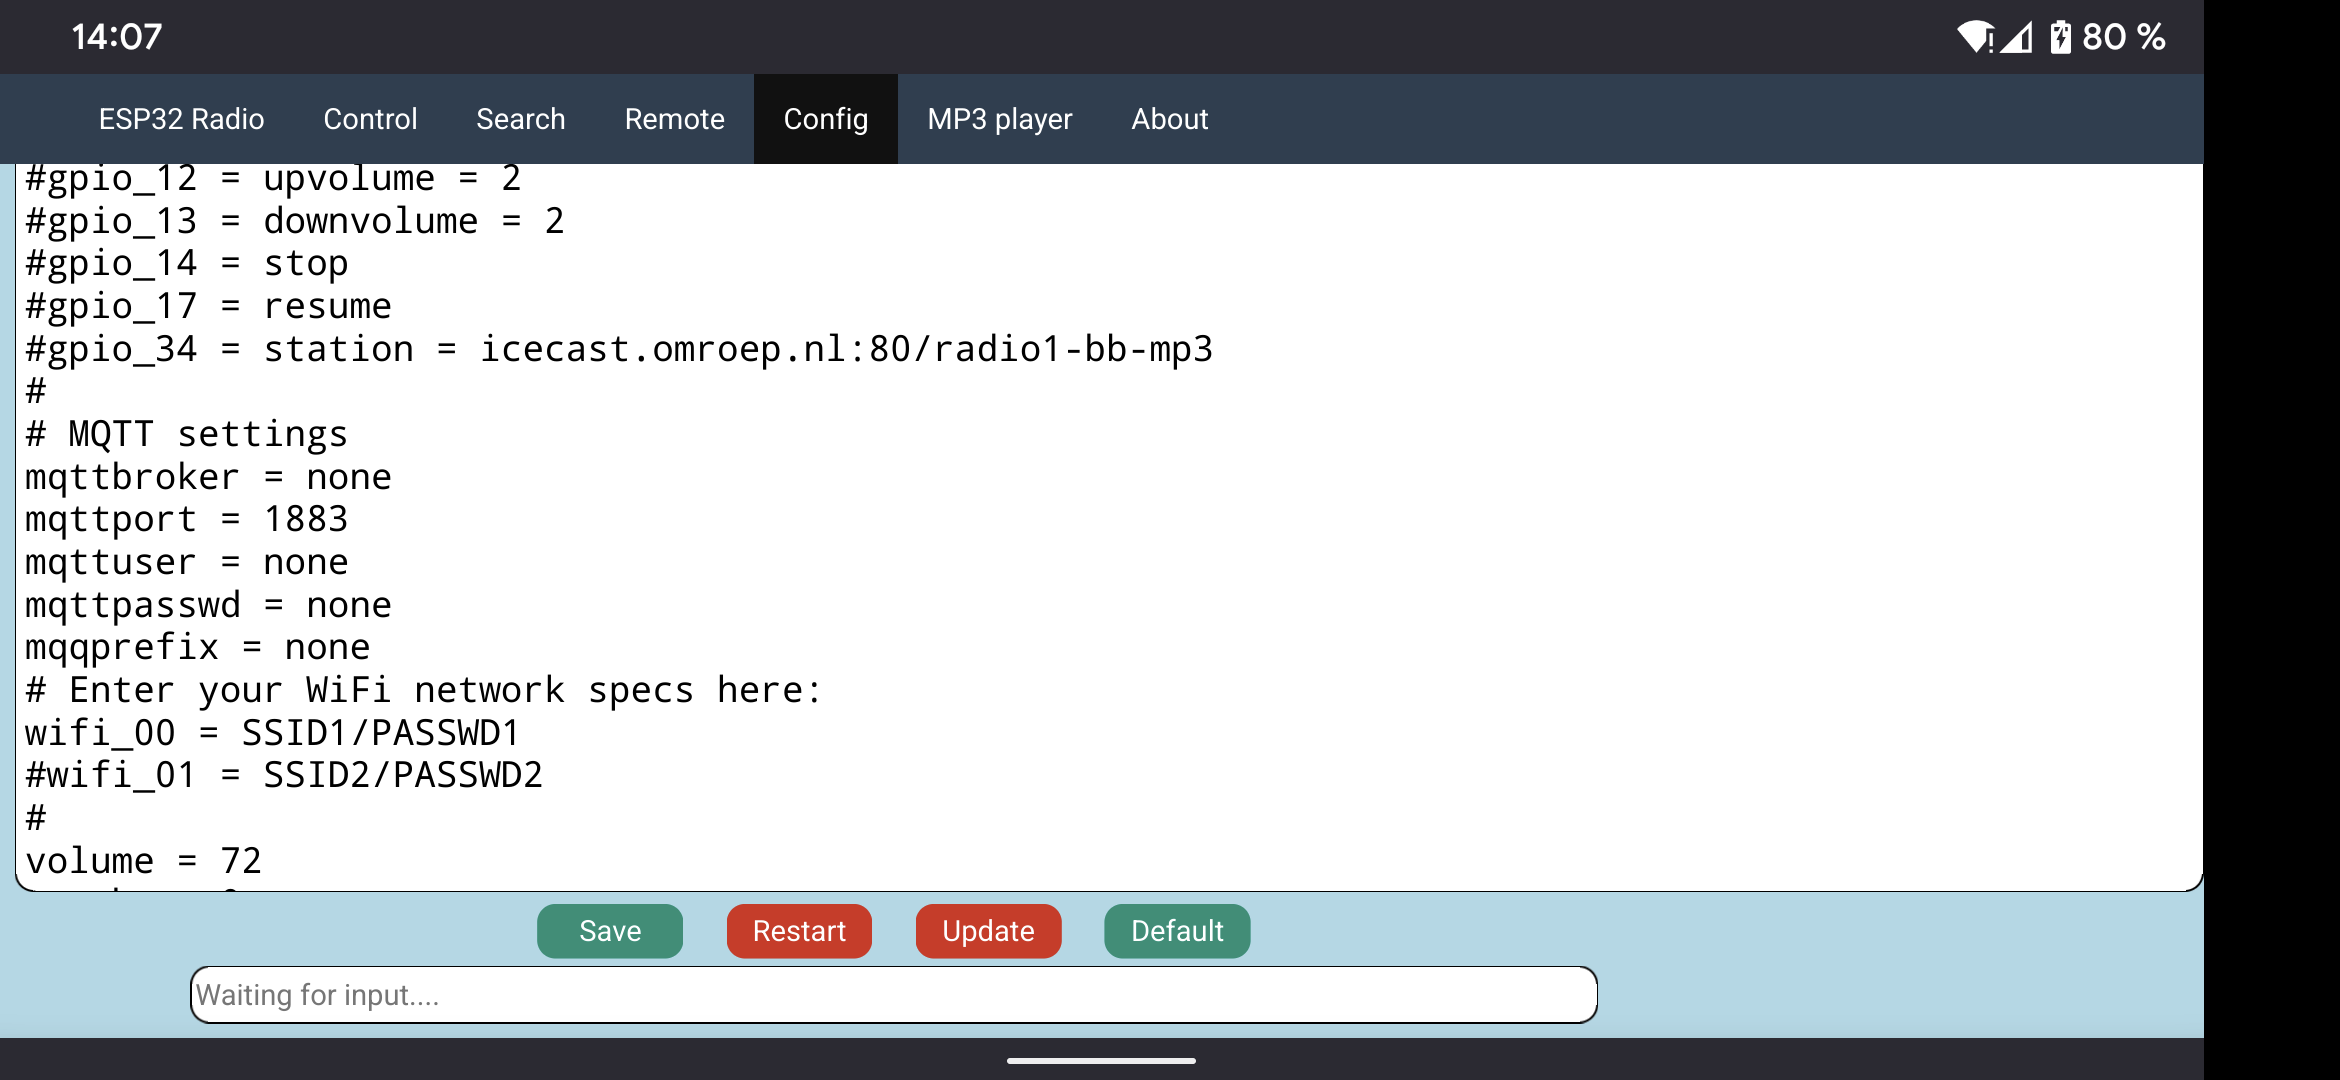
\includegraphics[width=\textwidth]{wlan2}};
\end{tikzpicture}
\caption{Defaults} \label{fig:1}
\end{figure}

Feld \emph{wifi\_00} W-Lan Namen und Passwort eingeben. "`Save"', "`Restart"' dr"ucken. Das Passwort wird auf dem ESP32 unverschl"usselt gespeichert!

\begin{figure}[H]
\centering
\begin{tikzpicture}
     \node[anchor=south west,inner sep=0] at (0,0) {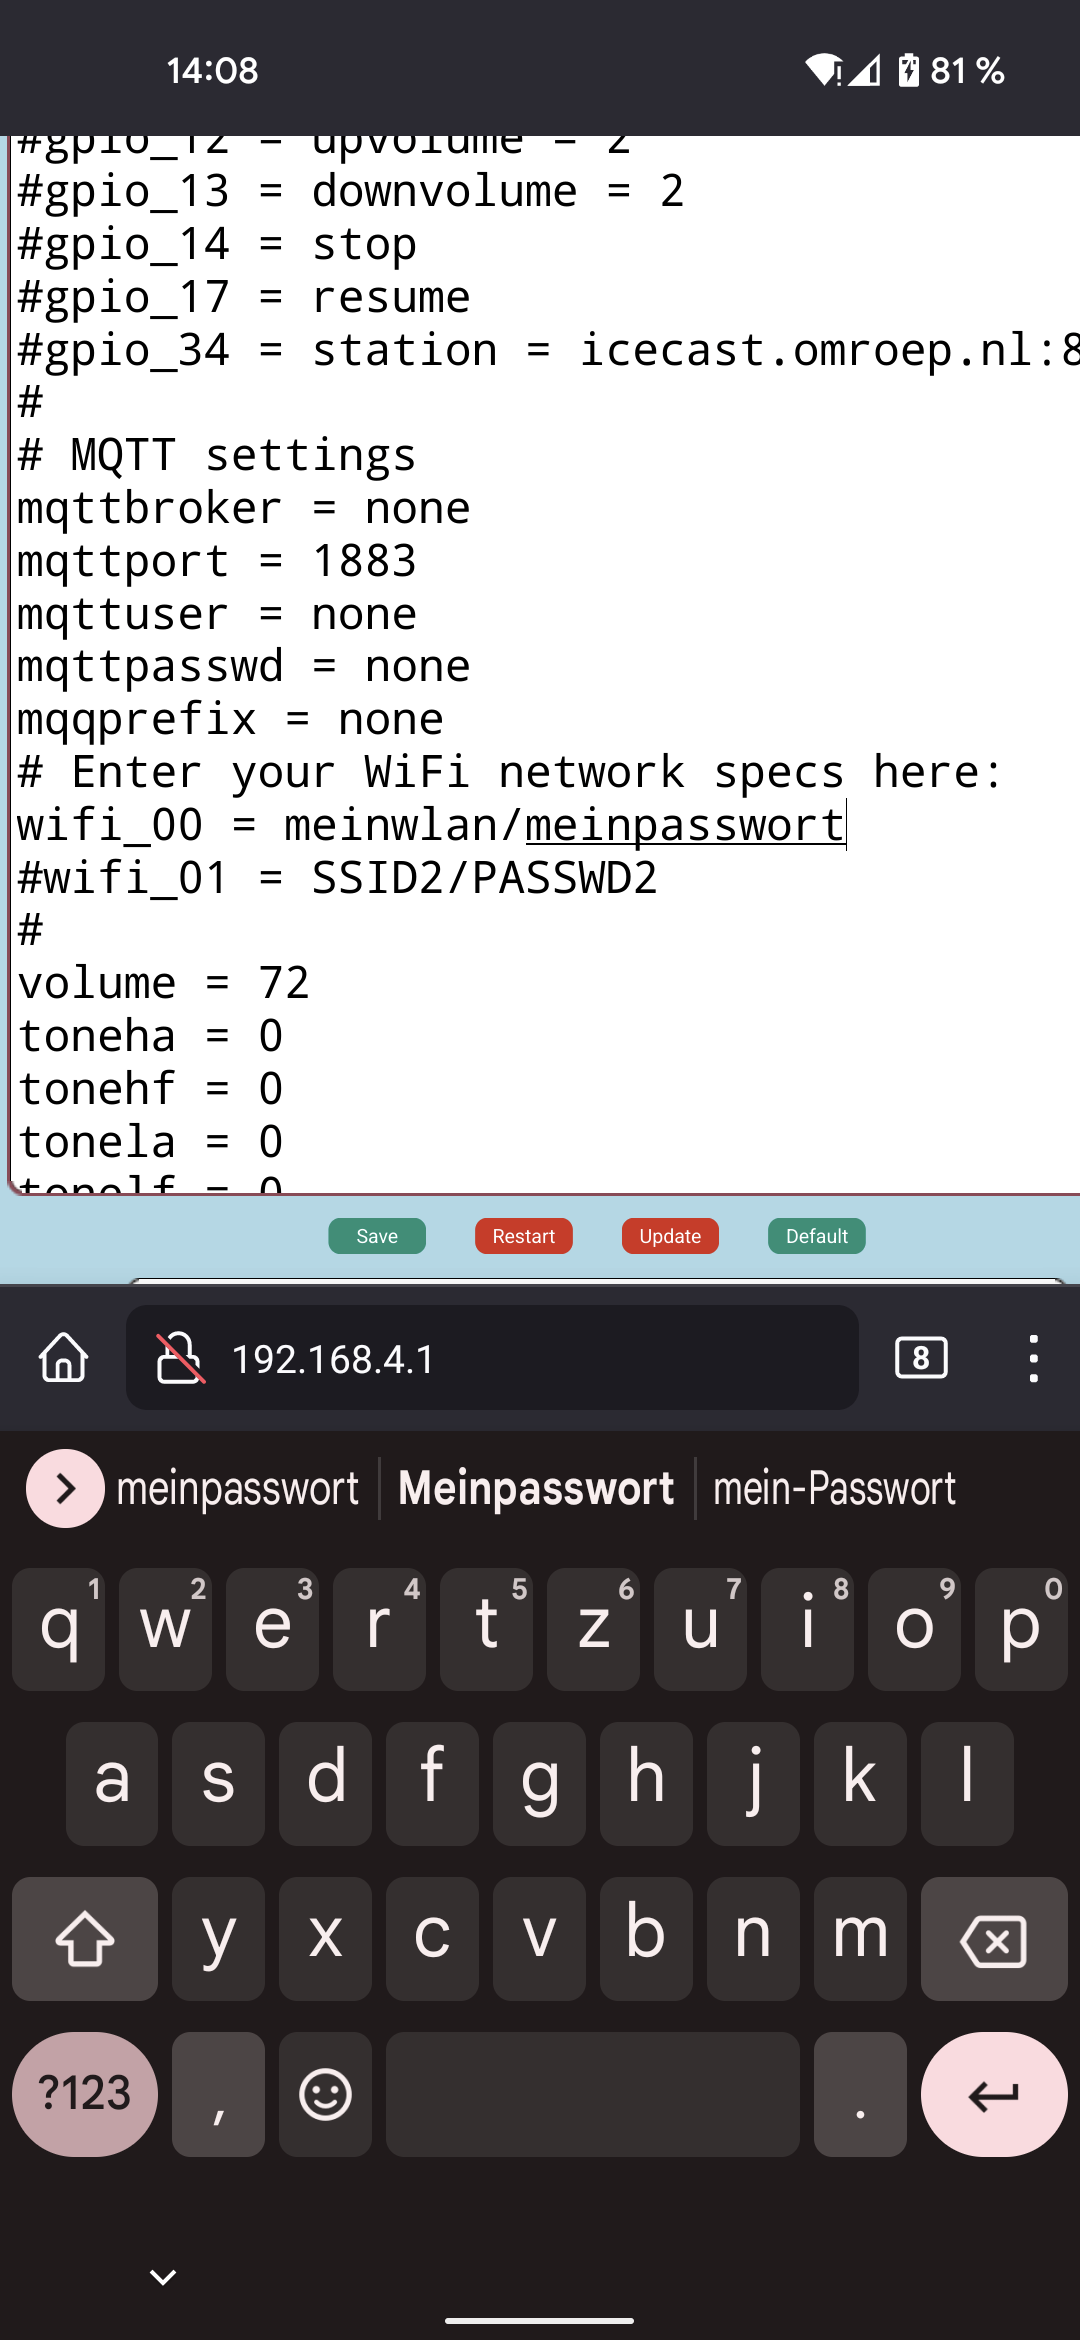
\includegraphics[width=.4\textwidth]{wlan3}};
\end{tikzpicture}
\caption{Passwort} \label{fig:1}
\end{figure}

Danach sollte sich der ESP32 im vorgegebenen W-Lan anmelden. Falls nicht, Terminalprogramm auf der USB seriellen Schnittstelle "offnen und Debugausgaben auswerten. Website aufrufen mit IP des ESP32 oder z.B. \emph{\href{http://esp32-arduino.fritz.box}{http://esp32-arduino.fritz.box}} falls man eine Fritzbox hat.\\
Das W-Lan wird immer ge"offnet wenn sich der ESP32 nicht in eines der vorgegebenen Netze einloggen kann.

\subsection{Webradio} \label{sec:bedienung:webradio}

Taste \textbf{TA} am Radio dr"ucken.

\textbf{Bedienung am Radio}

"Uber den Wippschalter der Automatik k"onnen am Webradio die Stationen ausgew"ahlt werden, wie im normalen Radiobetrieb. Die Automatiktaste kann bet"atigt ($\rightarrow$ Automatik Aus) sein.

\begin{itemize}
\item Wippschalter ganz links $\rightarrow$ Station "`1"' ausw"ahlen
\item Wippschalter links tippen $\rightarrow$ vorherige Station
\item Wippschalter rechts tippen $\rightarrow$ n"achste Station
\item Wippschalter ganz rechts $\rightarrow$ \todo nicht belegt
\end{itemize}

\textbf{Bedienung Webinterface}

Nach dem "Offnen der Webseite stehen alle Grundfunktionen zur Verf"ugung.

\begin{figure}[H]
\centering
\begin{tikzpicture}
     \node[anchor=south west,inner sep=0] at (0,0) {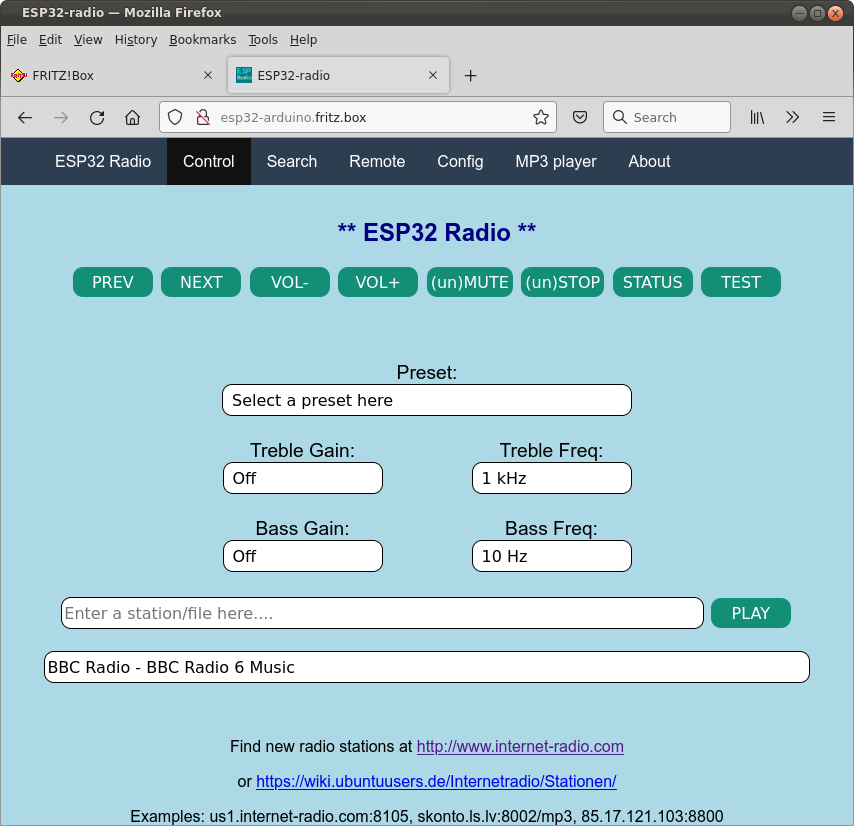
\includegraphics[width=.6\textwidth]{webradio1}};
\end{tikzpicture}
\caption{Webradio} \label{fig:1}
\end{figure}

Im Feld "`Enter a station/file here..."' kann die URL einer Radiostation angegeben und mit \emph{Play} gestartet werden. Geht nur ohne Protokollangabe (http://der URL weglassen). Es k"onnen nur unverschl"usselte Stationen wiedergegeben werden (kein https://). Die meisten Stationen unterst"utzen unverschl"usselte "Ubertragung, auch wenn es nicht explizit angegeben ist.

"Uber den Reiter \emph{Search} steht eine nach Musikrichtung sortierte Auswahl an Radiostationen zur Verf"ugung. Ausw"ahlen durch Anklicken, danach wird der Stream gestartet. Nicht alle funktionieren immer.

\subsection{Fernbedienung} \label{sec:bedienung:fernbedienung}

Rundfunkband am Radio ausw"ahlen. Webseite Reiter \emph{Remote} ausw"ahlen.

\begin{figure}[H]
\centering
\begin{tikzpicture}
     \node[anchor=south west,inner sep=0] at (0,0) {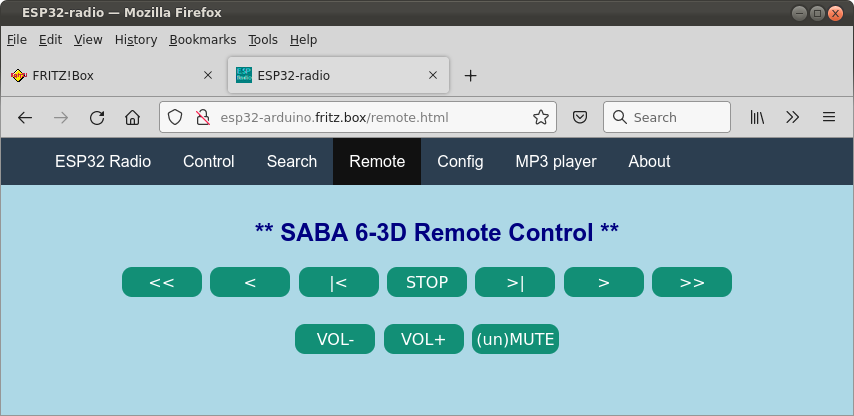
\includegraphics[width=.6\textwidth]{webradio2}};
\end{tikzpicture}
\caption{Fernbedienung} \label{fig:1}
\end{figure}

Bedienung entspricht dem Wippschalter am Ger"at. \textbf{|<} und \textbf{>|} starten einen Suchlauf. Falls aktueller Sender nicht verlassen wird die Taste gedr"uckt halten bis Sender verlassen wurde (so wie am Ger"at auch...).

\subsection{Einstellungen} \label{sec:bedienung:einstellungen}

Webseite Reiter \emph{Config} ausw"ahlen.

Es k"onnen die folgenden Einstellungen ge"andert werden:
\begin{itemize}
\item Uhrzeit / NTP
\item MQTT IoT 
\item Voreingestellte Radiosender. Diese Liste wird mit dem Wippschalter / dem \emph{Control} Reiter zur Verf"ugung gestellt
\item W-Lan Nutzer / Passwort
\end{itemize}

\begin{figure}[H]
\centering
\begin{tikzpicture}
     \node[anchor=south west,inner sep=0] at (0,0) {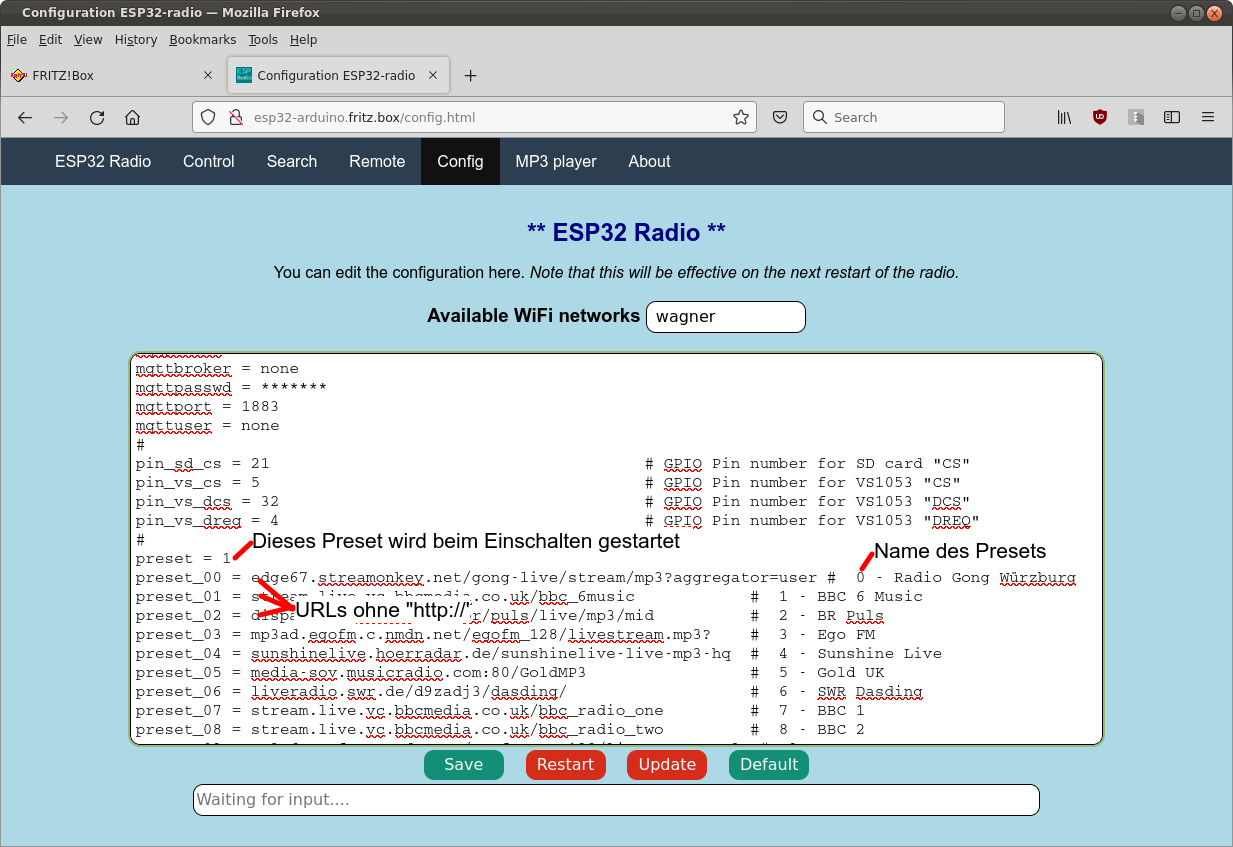
\includegraphics[width=\textwidth]{webradio3}};
\end{tikzpicture}
\caption{Konfiguration} \label{fig:config}
\end{figure}

Einstellunge "ubernehmen mit "`Save"', "`Restart"'.

\subsection{Weitere Funktionen}

Weitere Funktionen sind in der Dokumentation des ESP32-radio Projekts beschrieben.

\subsection{OTA Firmwareupdate}

Webseite Reiter \emph{Config} ausw"ahlen. \emph{Update} dr"ucken, siehe Bild \ref{fig:config}. Es wird die Datei \url{http://martinwag.atwebpages.com/ESP32_radio/firmware.bin} gepr"uft, heruntergeladen und ins Flash geschrieben\footnote{Download per HTTP. Keine Verschl"usselung, keine Authentifizierung, etc. .}. Das Kommando wird im Textfeld best"atigt, eine Erfolgsmeldung gibt es nicht. Sp"atestens nach ein paar Minuten sollte das Update fertig sein, im Reiter \emph{About} sollte eine neues Builddatum auftauchen (oder auch nicht falls kein Update verf"ugbar ist). 

Die Einstellungen werden beim Update beibehalten.

MD5 Version "`Build: 2022-08-08 -- 1"': c14b029a3c16b14e4aa896f9e22090a8.

\section{Schaltungsbeschreibung} \label{sec:schaltung}

Die Schaltung besteht aus folgenden Bl"ocken:
\begin{itemize}
\item Microcontroller ESP32 auf Daughterboard
\item Audioschaltung
\item Radio steuern per Webradio
\item Webradio steuern per Radio
\item Spannungsversorgung
\item Schnittstellen
\end{itemize}

In den folgenden Kapiteln wird Design, Funktion und Zusammenwirken beschrieben.

\subsection{Datenbl"atter} \label{sec:schaltung:datenblaetter}

Folgende Datenbl"atter und Application Notes wurden verwendet (u.A):
\begin{itemize}
\item ADA4522-1/ADA4522-2/ADA4522-4 Rev. F
\item AD8655/AD8656 Rev. E
\item VS1053b Datasheet Version: 1.31, 2017-11-17
\item VS10XX AppNote Rev 1.25
\item vs1033example\_rev07
\item Layout Considerations VS10XX AppNote Rev 1.0
\item DOIT ESP32 Devkit V1
\item ESP32­WROOM­32D \& ESP32­WROOM­32U Datasheet Version 2.0 2020
\item TI LM139, LM239, LM339, LM139A LM239A, LM339A, LM2901, LM2901AV, LM2901V  SLCS006U – OCTOBER 1979 – REVISED NOVEMBER 2018
\end{itemize}

\subsection{Microcontroller} \label{sec:schaltung:Microcontroller}

Der ESP32 wird verwendet da f"ur diesen mit dem ESP32-Radio ein passendes Softwareprojekt bereits zur Verf"ugung steht. Ebenfalls m"oglich w"are ein Raspberry Pi o."a. gewesen, dieser h"atte aber erheblich h"ohere Anforderungen an die Leistung des Netzteils gestellt.\\

Es wird ein vorgefertigtes Board verwendet.
\begin{itemize}
\item Sichere Funktion durch vorgefertige Platine, inkl. Netzteil, Resetbeschaltung und Programmierschaltung. Leichtes Pr"ufen da tauschbar.
\item ESP32-WROOM-32 Aufl"otmodul hat Pad auf Unterseite, somit nur umst"andlich handl"otbar.
\item Belegt weniger Platz auf Baseboard.
\item Programmieren ohne Baseboard m"oglich.
\item Vernachl"assigbarer Aufpreis.
\end{itemize}

\subsection{Audioschaltung} \label{sec:schaltung:audio}

\textbf{Codec}

Die Audioschaltung basiert auf einem VLSI VS1053 MP3 Hardware Codec. Wir nutzen nur den Decoder. Der VS1053 wird vom ESP32-Radio Projekt vorgegeben. Schaltung und Layout sind nach Application Note von VLSI.

\textbf{Verst"arker}

Das vomn VS1053 ausgegebene Audiosignal wird von einem Audioverst"arker verst"arkt. Dies erm"oglicht ein Anpassen des Audiopegels an die Empfindlichkeit des TA Eingangs. \\
Der OP ist als \emph{\href{https://www.mikrocontroller.net/articles/Operationsverst\%C3\%A4rker-Grundschaltungen\#Betrieb\_mit\_einfacher\_Versorgungsspannung}{nichtinvertierender Wechselspannungsverstärker mit einfacher Versorgungsspannung}} verschaltet. Die Schaltung ist dimensioniert um einen hochohmigen Eingang zu treiben. Der OP muss folgende Bedingungen erf"ullen:
\begin{itemize}
\item Betrieb an 5\,V einfacher Versorgung
\item Linear im Audiobereich
\item Ausgangsspannung bis ca. +/- 0,5\,V an Versorgungsspannungen
\end{itemize}
Es sind somit praktisch alle f"ur niedrige Versorgungsspannungen optimierten OPs geeignet.

\textbf{Massef"uhrung}

Die Analogschaltung verwendet die allgemeine Massefl"ache (keine Sternanbindung). Die Schaltung ist nicht mit der Masse des Radios verbunden.

\textbf{Ausgangstrafo}

Um Brummen zu vermeiden muss die Audioschaltung am GND Anschluss TA mit dem Radio verbunden werden. Gleichzeitig muss aber der Versorgungsstrom der Mikrocontrollerschaltung "uber den Fernbedienungsanschluss flie"sen. Diese Aufteilung ist nur m"oglich wenn entweder die Versorgungsseite oder die Audioseite potentialgetrennt werden. Schaltung Rev. A hat einen DC/DC Wandler vorgesehen, dieser hat den Radioempfang gest"ort. Schaltung Rev. B verwendet daher einen Ausgangstrafo.

\textbf{Stereo}

Die Audioschaltung ist zweikanalig ausgef"uhrt. Bei der Platinenbest"uckung kann ausgew"ahlt werden ob am Ausgang beide Signale zu einem Monosignal gemischt werden oder Stereo ausgegeben wird. Dies erm"oglicht eine einfache Anpassung zur Verwendung an Stereoger"aten.

\subsection{Steuerung Radio} \label{sec:schaltung:steuern-radio}

Der Steuerteil ersetzt 1:1 die kabelgebundene SABA Fernbedienung. Die Schaltung basiert auf der IR Fernbedienung Saba Freiburg 125 von H. Krebs. Schaltung und Bauteilwerte wurde an die 6-3D Serie angepasst.

\textbf{Automatik Steuerung}

Bildet die Schaltung in der Fernbedienung nach. Die Widerst"ande 1\,kOhm sind leistungstechnisch so ausgelegt das sie bei Softwarefehler (alle drei Relais geschaltet) nicht zerst"ort werden.

\textbf{Haltespule}

In der SABA Fernbedienung entspricht die Haltespule einem Relais mit Selbsthaltung. Wenn ein Sender gefunden ist flie"st kein Strom mehr und die Spule f"allt ab. Die Schaltung und Software muss dieses Verhalten nachbilden:
\begin{itemize}
\item Das Radio muss weiterhin einen Widerstand ca. 6\,kOhm "`sehen"'\footnote{Siehe Schaltschema SABA - Fernbed. Anschl.} da die im Radio verbaute Haltespule sonst nicht mehr funktioniert
\item Die Software muss Abfall des Stromflusses erkennen ("`Sender gefunden"') und Suchlaufrelais abschalten.
\end{itemize}
Es muss ein Widerstand mind. 0,25\,W verwendet werden.

\textbf{Lautst"arke, Stummschaltung}

Im Gegensatatz zur Schaltung von H. Krebs verwenden wir Relais. Die zus"atzlichen Kontakte werden zur Verriegelung verwendet. Dies verhindert Zerst"orung des Radio Netztrafos durch Kurzschluss bei Softwarefehler (Relais laut und leise gleichzeitig geschaltet). Es verhindert auch gleichzeitigen Betrieb von Suchlauf und Stummschaltung.

\textbf{Netzschalter}

Der Schaltungsteil Netzschalter ist optional. Er erm"oglicht ein Ausschalten (und bei USB Versorgung auch Einschalten) des Radios per Webradio. Falls nicht ben"otigt, Spannung 230\,V AC auf N1 oder N2 br"ucken. Alternativ kann auch die eine H"alfte des Zentrierstiftes aus \ref{sec:aufbau:anschlussstecker} abgeschliffen werden um den Schaltkontakt im Radio dauerhaft geschlossen zu halten. Die zugeh"origen Kontaktstifte k"onnen dann entfallen.

Der Wechlser im Relais bildet in Verbindung mit dem Netzschalter im Radio eine Wechselschaltung. Um den Zustand auch ohne Versorgungsspannung zu halten wird ein bistabiles Relais verwendet.

\todo nicht in Software implementiert.

\textbf{USB Versorgung}

Optional, nur Sinnvoll in Verbindung mit Netzschalter, erm"oglicht Standby / Einschalten per Netzwerk. Der Schaltungsteil "`Spannungsversorgung 5\,V"'\footnote{Siehe Schaltplan Seite 3} und der Ausgangstrafo kann entfallen.

\textbf{Infrarotfernbedienung}

Wird vom ESP32-radio Projekt unterst"utzt, nicht weiter getestet. Funktion wird in der Doku des ESP32-radio detailliert beschrieben.

\subsection{Steuerung Webradio} \label{sec:schaltung:steuern-web}

Der Schaltungsteil Steuerung Webradio erm"oglicht eine Bedienung des Webradios mit der Suchlaufwippe am Radio. Diese hat f"unf Schalterstellungen:
\begin{itemize}
\item Nicht bet"atigt
\item Suchlauf jeweils links und rechts.
\item Schnelllauf jeweils links und rechts
\end{itemize}
Abh"angig von der Schalterposition wird das Signal auf der Suchlaufleitung ver"andert:
\begin{itemize}
\item Keine Bet"atigung - DC Vorspannung der Triode EABC80 R"o. 4.
\item Bet"atigung Suchlauf - DC Spannung wird negativ verschoben (Stummschaltung), AC wird aufaddiert. AC Phase abh. von der Laufrichtung.
\item Bet"atigung Schnelllauf - Wie Suchlauf, aber AC Amplitude h"oher.
\end{itemize}

Die Schalterposition kann folglich anhand der aufaddierten Wechselspannung ermittelt werden. Der Verlauf wird an der Simulation sichtbar:

\begin{itemize}
\item 1\,s ... 2\,s - links Schnelllauf
\item 3\,s ... 4\,s - links Suchlauf
\item 7\,s ... 8\,s - rechts Schnelllauf
\item 9\,s ... 10\,s - rechts Suchlauf
\item restliche Zeit - nicht bet"atigt.
\end{itemize}

\begin{figure}[H]
\centering
\begin{tikzpicture}
     \node[anchor=south west,inner sep=0] at (0,0) {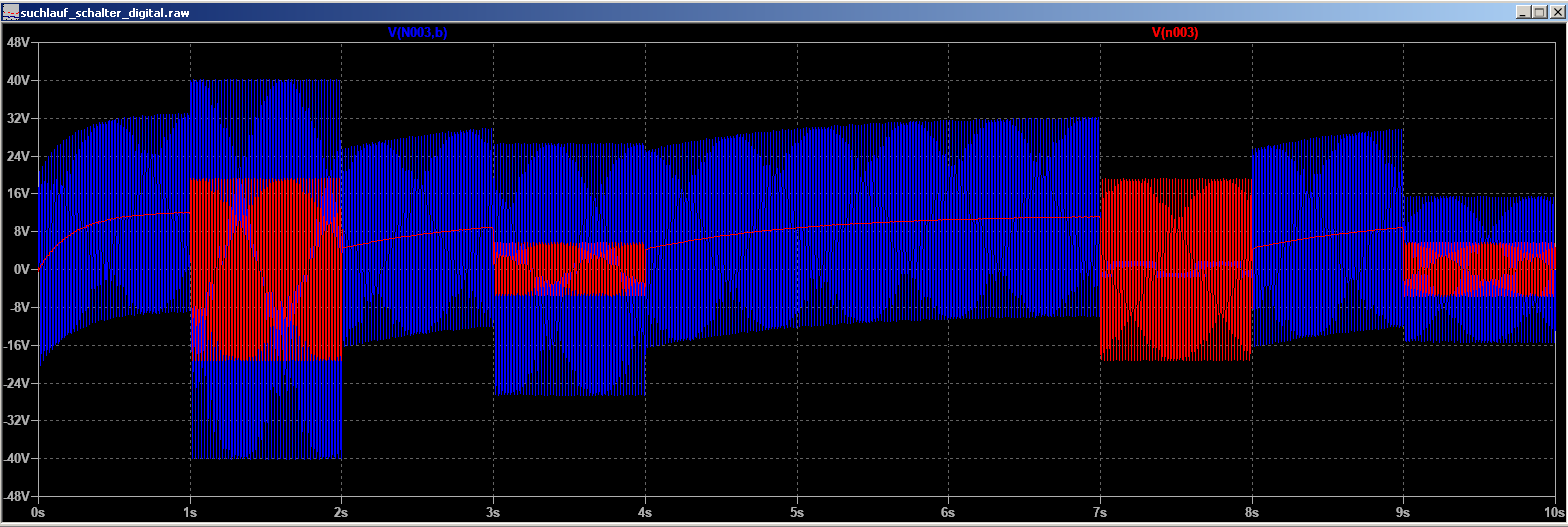
\includegraphics[width=\textwidth]{messen.png}};
\end{tikzpicture}
\caption{Spannung Rot: Suchlaufleitung -- AC 0V, Blau: Suchlaufleitung -- AC 15V -90°} \label{fig:1}
\end{figure}

Messung mit Einweggleichrichtung und Siebung der Wechselspannung. Umsetzung in digitale Signale mit Komparatoren. Die Spannungen beziehen sich auf die Mittelanzapfung des Trafos. Dieser Punkt ist \textbf{nicht} mit der Masse des Radios verbunden. Daher ist f"ur die digitalen Signale Potentialtrennung erforderlich.

\section{Untersuchungen} \label{sec:untersuchung}

\subsection{Probleme} \label{sec:untersuchung:probleme}

Probleme und L"osungsvorschl"age.

\textbf{In Software funktioniert \emph{xyz} nicht}

\begin{itemize}
\item ESP32 mit PC USB verbinden, Kapitel \ref{sec:aufbau:programmierung} beachten. Der ESP32 verh"alt sich wie ein USB Seriell Wandler.
\item Serielles Terminal verbinden, 115200 8-N-1. Linux z.B. minicom, Windows z.B. Putty oder HyperTerminal
\item Funktion starten, Ausgabe auswerten. 
\item Im Terminal k"onnen auch Kommandos eingegeben werden (z.B. \emph{reset}). Der ESP32 selbst macht kein "`Echo"', d.H. abh"angig von der Terminalkofiguration sieht man die eigene Eingabe nicht. "`Enter"' f"uhrt Eingabe aus. Liste der Kommandos ist im Sourcecode in "`main.c"', Funktion "`analyzeCmd"' enthalten.
\end{itemize}

\textbf{Erkennung TA Eingang und LEDs in den Tasten}

Die Gl"uhlampen f"ur die Taster werden nicht mehr hergestellt und sind auch anderweitig nicht auftreibbar. Werden diese durch LED + Gleichrichter ersetzt funktioniert die Schaltung zur Erkennung des TA nicht mehr. Diese kann wie folgt angepasst werden

\begin{figure}[H]
\centering
\begin{tikzpicture}
     \node[anchor=south west,inner sep=0] at (0,0) {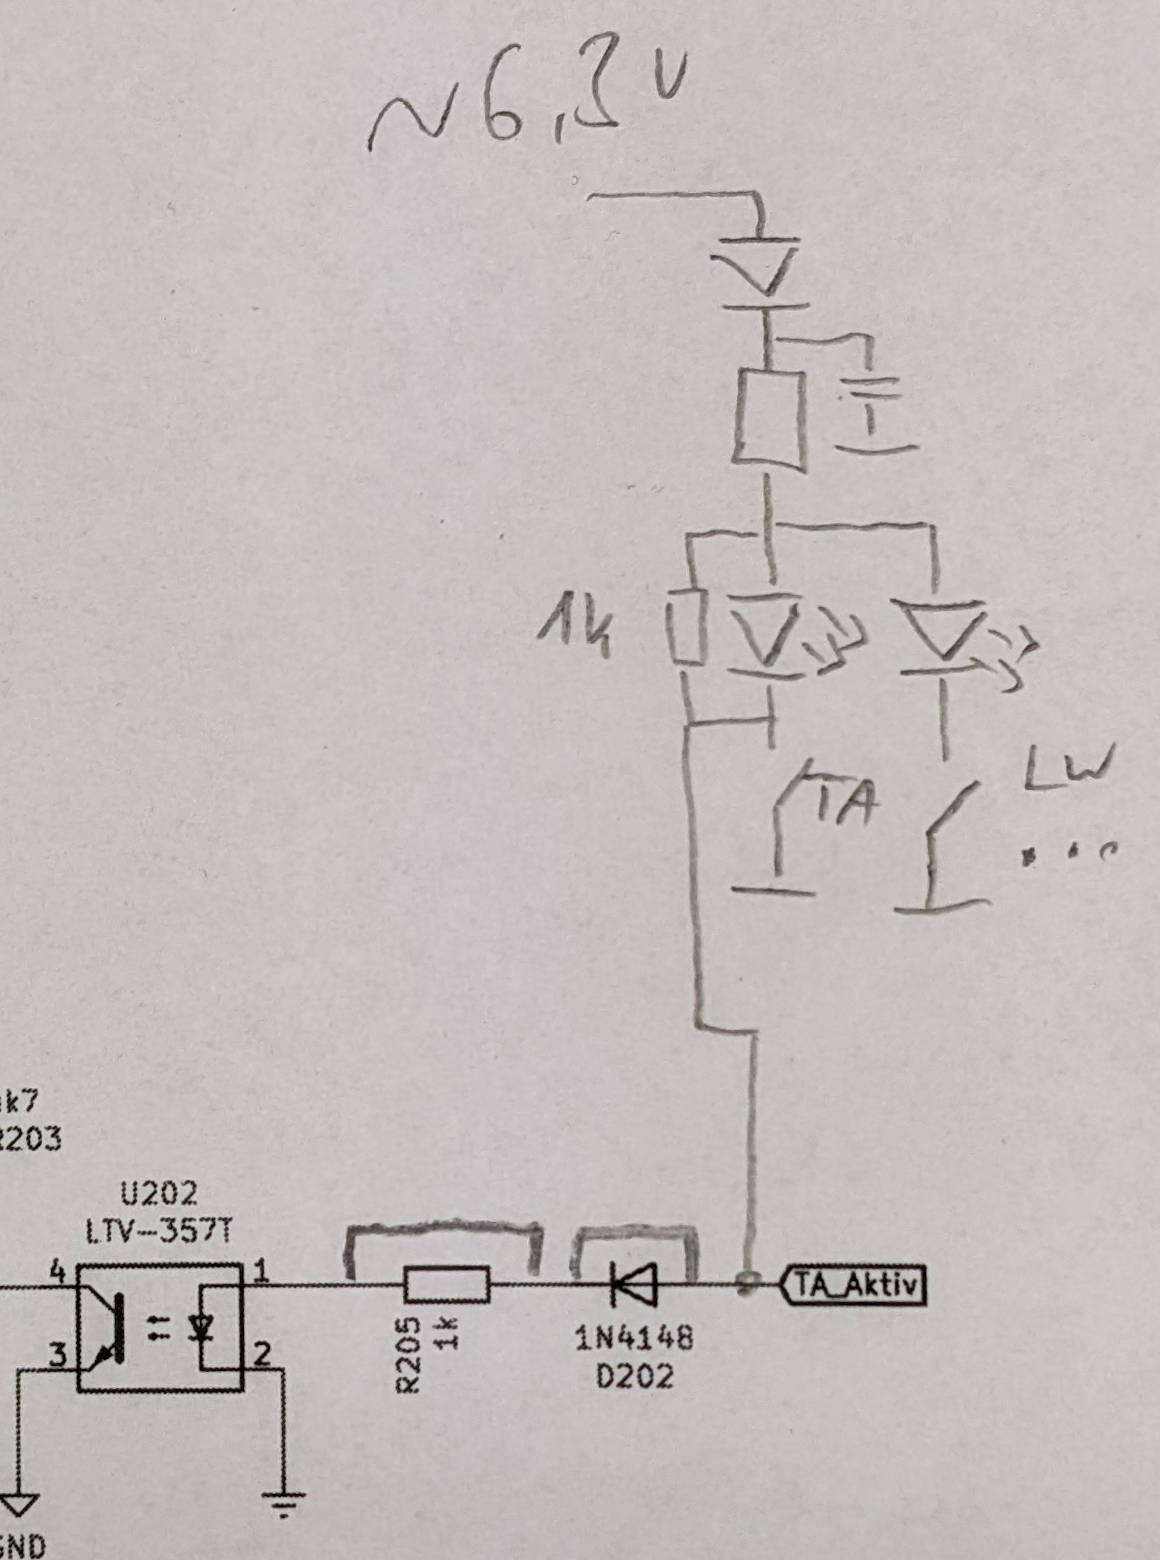
\includegraphics[width=.325\textwidth]{led1}};
\end{tikzpicture}
\hspace{1cm} %no empty line!
\begin{tikzpicture}
     \node[anchor=south west,inner sep=0] at (0,0) {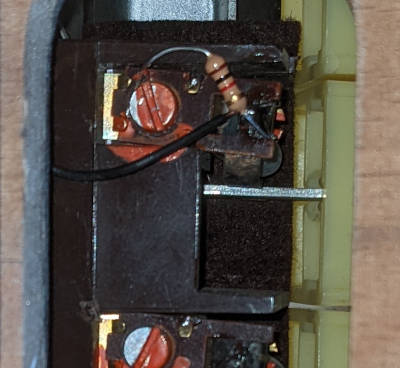
\includegraphics[width=.47\textwidth]{led2}};
\end{tikzpicture}
\caption{Anpassung LEDs} \label{fig:1}
\end{figure}

\textbf{Webinterface reagiert langsam}

Webseite aufrufen mit der IP Adresse statt URL. Scheinbar bringen div. Router da etwas durcheinander wenn mehrere ESP32 am Netz sind.

\textbf{Weitere}

\todo weitere ...

\subsection{Ausgangs"ubertrager} \label{sec:untersuchung:ausgangsuebertrager}

Wir haben einen relativ niederohmigen Ausgang (Opamp) und eine sehr hochohmige Last (Radio Phonoeingang).

Es wurden verschiedene Ausgangs"ubertrager untersucht um ein geeignetes Bauteil zu finden. 

Von links nach rechts:
\begin{itemize}
\item Ground Loop Isolator Sinus Live GL-205, 2 x RCA (ca. 15 Euro)
\item Telefon"ubertrager 600:600 Ohm EI14 (Ebay China ca. 4 Euro / 10 Stk.)
\item CMC 47\,mH Talema CAF 0,5-47 (ca. 3 Euro)
\item NFU 1-1 EI19 50\,Hz ... 10\,kHz, 34\,mH (ca. 3 Euro)
\item FeinTech ATG00101 Audio Masse-Trennglied, Klinke 3,5\,mm (ca. 15 Euro)
\end{itemize}

Wir brauchen ca. 100\,Hz ... 15\,kHz.

Versuchsaufbau nach \emph{\href{https://keysightoscilloscopes.wordpress.com/2016/04/13/how-to-create-bode-plots-on-an-oscilloscope/}{Vorschlag Keysight, how to create bode plots on an oscilloscope}}.

Sweep 0 ... 20\,kHz, 1\,V\textsubscript{SS}, 50\,Ohm Ausgangswiderstand Generator, 100\,kOhm Lastwiderstand Sekund"arseite. Scheinbar hat der Generator hier einen Bug, es kommen 2\,V\textsubscript{SS} raus?

\begin{figure}[H]
\centering
\begin{tikzpicture}
     \node[anchor=south west,inner sep=0] at (0,0) {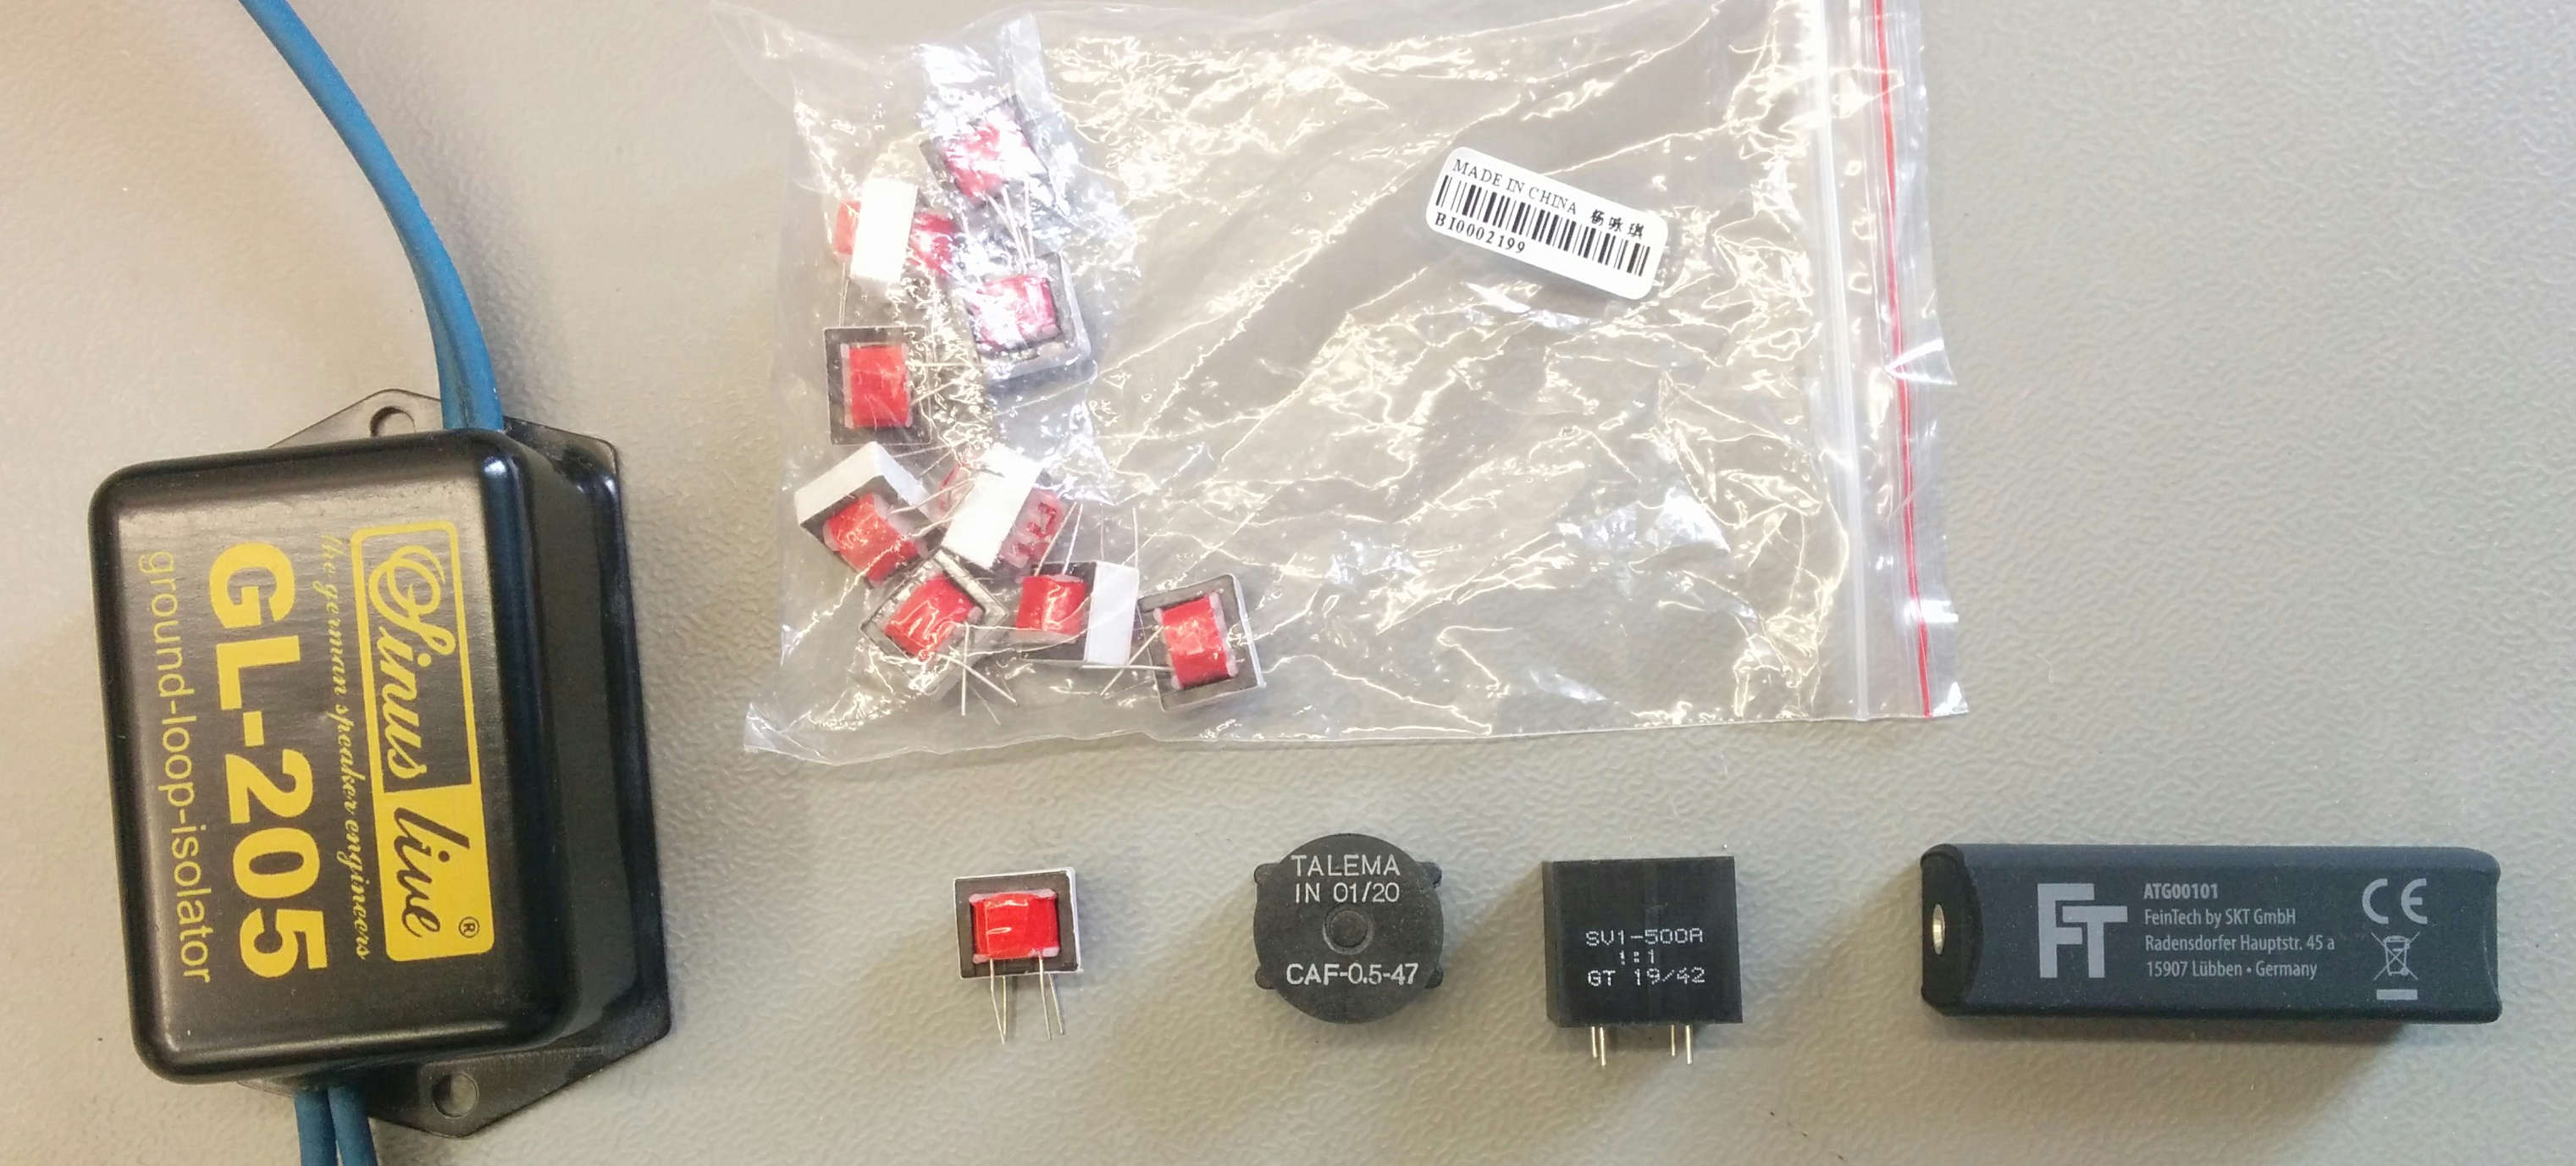
\includegraphics[width=\textwidth]{uebertrager.jpg}};
\end{tikzpicture}
\caption{getestete "Ubertrager} \label{fig:1}
\end{figure}

\begin{figure}[H]
\centering
\begin{tikzpicture}
     \node[anchor=south west,inner sep=0] at (0,0) {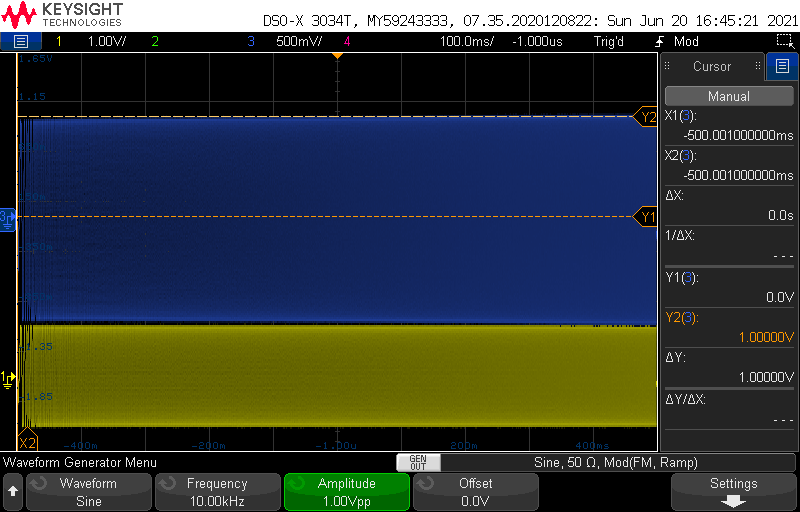
\includegraphics[width=\tscopesize]{image13017.png}};
\end{tikzpicture}
\caption{GL-205} \label{fig:1}
\end{figure}

\begin{figure}[H]
\centering
\begin{tikzpicture}
     \node[anchor=south west,inner sep=0] at (0,0) {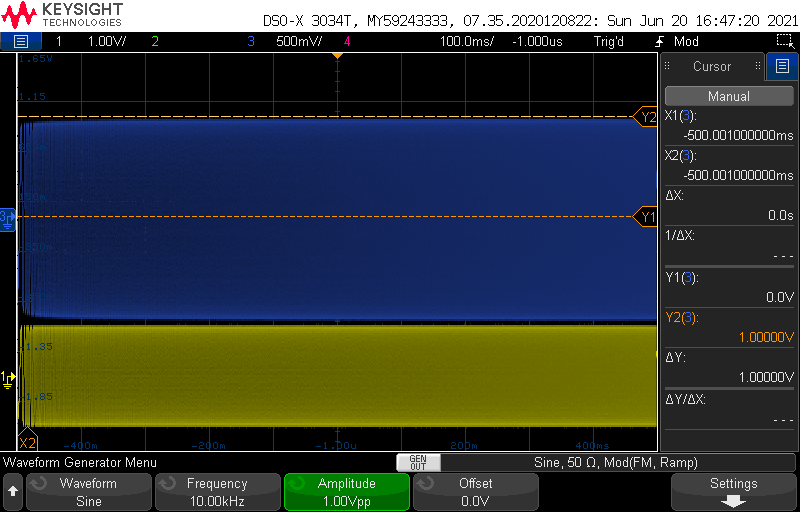
\includegraphics[width=\tscopesize]{image5878.png}};
\end{tikzpicture}
\caption{China 600:600 Ohm} \label{fig:1}
\end{figure}

\begin{figure}[H]
\centering
\begin{tikzpicture}
     \node[anchor=south west,inner sep=0] at (0,0) {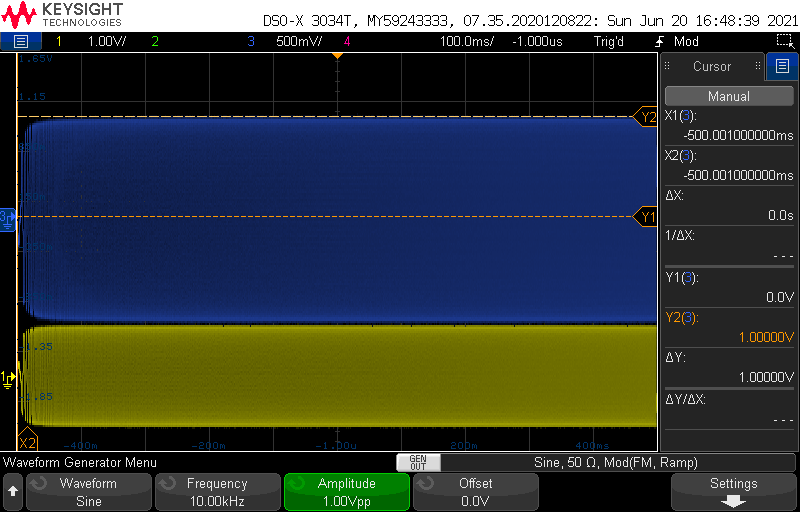
\includegraphics[width=\tscopesize]{image3233.png}};
\end{tikzpicture}
\caption{CMC 47\,mH} \label{fig:1}
\end{figure}

\begin{figure}[H]
\centering
\begin{tikzpicture}
     \node[anchor=south west,inner sep=0] at (0,0) {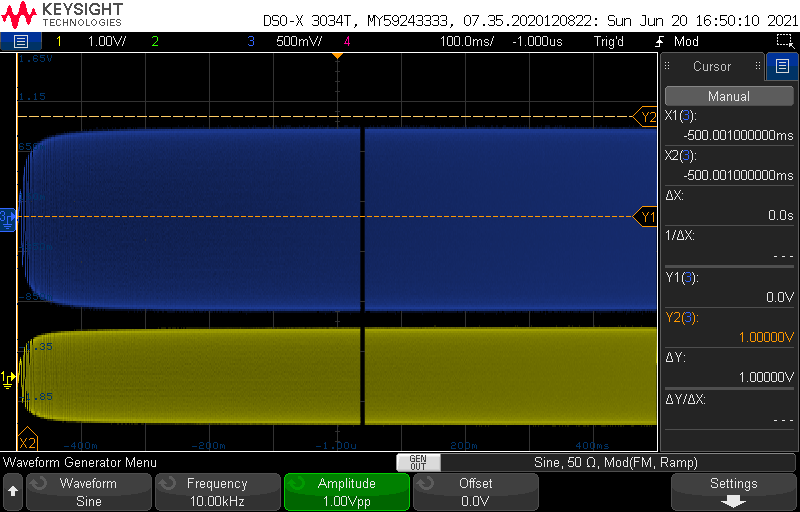
\includegraphics[width=\tscopesize]{image5900.png}};
\end{tikzpicture}
\caption{NFU 1-1} \label{fig:1}
\end{figure}

\begin{figure}[H]
\centering
\begin{tikzpicture}
     \node[anchor=south west,inner sep=0] at (0,0) {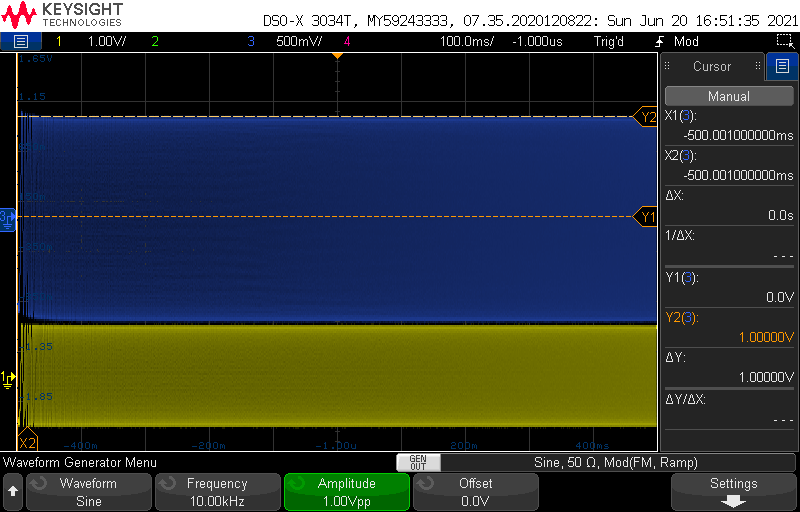
\includegraphics[width=\tscopesize]{image20292.png}};
\end{tikzpicture}
\caption{ATG00101} \label{fig:1}
\end{figure}

Im niedrigen Frequenzbereich sind Unterschiede sichtbar. Daher nochmal Detailmessung 0 ... 2\,kHz.

\begin{figure}[H]
\centering
\begin{tikzpicture}
     \node[anchor=south west,inner sep=0] at (0,0) {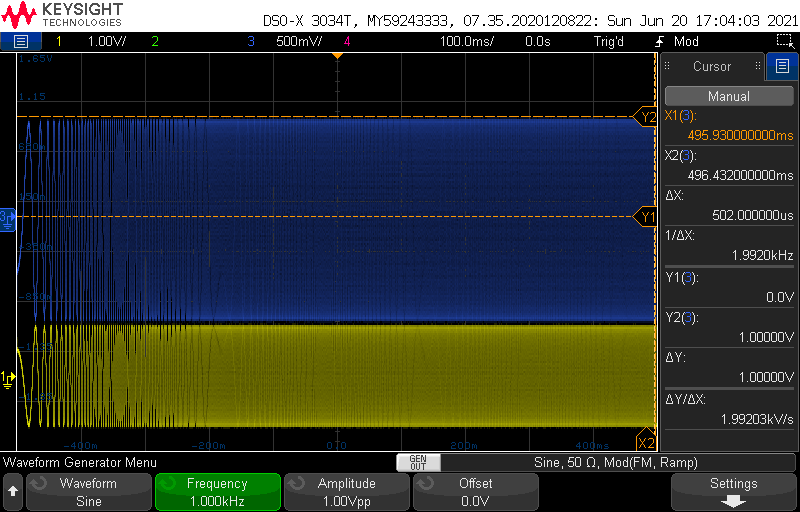
\includegraphics[width=\tscopesize]{image5940.png}};
\end{tikzpicture}
\caption{GL-205} \label{fig:1}
\end{figure}

\begin{figure}[H]
\centering
\begin{tikzpicture}
     \node[anchor=south west,inner sep=0] at (0,0) {\includegraphics[width=\tscopesize]{image923.png}};
\end{tikzpicture}
\caption{China 600:600 Ohm} \label{fig:1}
\end{figure}

\begin{figure}[H]
\centering
\begin{tikzpicture}
     \node[anchor=south west,inner sep=0] at (0,0) {\includegraphics[width=\tscopesize]{image30564.png}};
\end{tikzpicture}
\caption{CMC 47\,mH} \label{fig:1}
\end{figure}

\begin{figure}[H]
\centering
\begin{tikzpicture}
     \node[anchor=south west,inner sep=0] at (0,0) {\includegraphics[width=\tscopesize]{image4312.png}};
\end{tikzpicture}
\caption{NFU 1-1} \label{fig:1}
\end{figure}

\begin{figure}[H]
\centering
\begin{tikzpicture}
     \node[anchor=south west,inner sep=0] at (0,0) {\includegraphics[width=\tscopesize]{image9178.png}};
\end{tikzpicture}
\caption{ATG00101} \label{fig:1}
\end{figure}

Ergebnis:
\begin{itemize}
\item Die beiden kommerziell erhältlichen Massetrenner zeigen keinen nennenswerten Unterschied zwischen dem Spannungspegel an Ein- und Ausgang.
\item Bei niedrigen Ausgangsfrequenzen wird ggf. X\textsubscript{L} zu niedrig? $\rightarrow$ Stromfluss.
\item Die CMC funktioniert "uberraschend gut -- in diesem Testaufbau sogar besser als der Audio"ubertrager.
\item Der 600:600 Ohm Telefon"ubertrager ist mehr als ausreichend gut, billig, leicht zu bekommen und klein.
\end{itemize}

\subsection{W-Lan Antenne}

Es kann eine 2,4\,GHz W-Lan Antenne angeschlossen werden\footnote{\url{https://community.home-assistant.io/t/how-to-add-an-external-antenna-to-an-esp-board/131601}}.  

\begin{figure}[H]
\centering
\begin{tikzpicture}
     \node[anchor=south west,inner sep=0] at (0,0) {\includegraphics[width=.4\textwidth]{ant1}};
\end{tikzpicture}
\hspace{1cm} %no empty line!
\begin{tikzpicture}
     \node[anchor=south west,inner sep=0] at (0,0) {\includegraphics[width=.434\textwidth]{ant2}};
\end{tikzpicture}
\caption{Nach Anleitung} \label{fig:1}
\end{figure}

Anstelle eines Kabels kann auch eine Buchse montiert werden.

\begin{figure}[H]
\centering
\begin{tikzpicture}
     \node[anchor=south west,inner sep=0] at (0,0) {\includegraphics[width=.6\textwidth]{ant3}};
\end{tikzpicture}
\caption{Mit Buchse / Stecker} \label{fig:1}
\end{figure}
                                                        
Im Versuch wurde das Signal ca. 6 ... 10\,dB st"arker.

\appendix

\section{Ausgabe md5sum Webserver}

Version "`Build: 2022-08-08 -- 1"'

\begin{lstlisting}
martin@mint ~/workspace/esp32_radio/ESP32-Radio/Release $ wget http://martinwag.atwebpages.com/ESP32_radio/firmware.bin
--2022-08-08 16:10:38--  http://martinwag.atwebpages.com/ESP32_radio/firmware.bin
Resolving martinwag.atwebpages.com (martinwag.atwebpages.com)... 185.176.43.53
Connecting to martinwag.atwebpages.com (martinwag.atwebpages.com)|185.176.43.53|:80... connected.
HTTP request sent, awaiting response... 200 OK
Length: 937040 (915K) [application/octet-stream]
Saving to: firmware.bin.1

firmware.bin.1                     100%[================================================================>] 915,08K  3,88MB/s    in 0,2s    

2022-08-08 16:10:38 (3,88 MB/s) - firmware.bin.1 saved [937040/937040]

martin@mint ~/workspace/esp32_radio/ESP32-Radio/Release $ md5sum firmware.bin*
c14b029a3c16b14e4aa896f9e22090a8  firmware.bin
c14b029a3c16b14e4aa896f9e22090a8  firmware.bin.1
\end{lstlisting}


\section{Ausgabe esptool.py}

\begin{lstlisting}
$ esptool.py  erase_flash
esptool.py v4.1
Found 2 serial ports
Serial port /dev/ttyUSB0
Connecting.....
Detecting chip type... Unsupported detection protocol, switching and trying again...
Connecting.......
Detecting chip type... ESP32
Chip is ESP32-D0WDQ6 (revision 1)
Features: WiFi, BT, Dual Core, 240MHz, VRef calibration in efuse, Coding Scheme None
Crystal is 40MHz
MAC: ac:67:b2:36:b3:b4
Uploading stub...
Running stub...
Stub running...
Erasing flash (this may take a while)...
Chip erase completed successfully in 2.3s
Hard resetting via RTS pin...

$ esptool.py --chip esp32 --baud 921600 --before default_reset --after hard_reset write_flash -z --flash_mode dio --flash_freq 80m --flash_size detect 0xe000 /opt/eclipse/arduinoPlugin/packages/esp32/hardware/esp32/1.0.6/tools/partitions/boot_app0.bin 0x1000 /opt/eclipse/arduinoPlugin/packages/esp32/hardware/esp32/1.0.6/tools/sdk/bin/bootloader_dio_80m.bin 0x10000 /home/martin/workspace/esp32_radio/ESP32-Radio/Release/ESP32_Radio.bin 0x8000 /home/martin/workspace/esp32_radio/ESP32-Radio/Release/ESP32_Radio.partitions.bin 
esptool.py v4.1
Found 2 serial ports
Serial port /dev/ttyUSB0
Connecting......
Chip is ESP32-D0WDQ6 (revision 1)
Features: WiFi, BT, Dual Core, 240MHz, VRef calibration in efuse, Coding Scheme None
Crystal is 40MHz
MAC: ac:67:b2:36:b3:b4
Uploading stub...
Running stub...
Stub running...
Changing baud rate to 921600
Changed.
Configuring flash size...
Auto-detected Flash size: 4MB
Flash will be erased from 0x0000e000 to 0x0000ffff...
Flash will be erased from 0x00001000 to 0x00005fff...
Flash will be erased from 0x00010000 to 0x000f4fff...
Flash will be erased from 0x00008000 to 0x00008fff...
Compressed 8192 bytes to 47...
Wrote 8192 bytes (47 compressed) at 0x0000e000 in 0.1 seconds (effective 1005.8 kbit/s)...
Hash of data verified.
Compressed 17120 bytes to 11164...
Wrote 17120 bytes (11164 compressed) at 0x00001000 in 0.3 seconds (effective 460.0 kbit/s)...
Hash of data verified.
Compressed 936896 bytes to 530440...
Wrote 936896 bytes (530440 compressed) at 0x00010000 in 7.1 seconds (effective 1051.7 kbit/s)...
Hash of data verified.
Compressed 3072 bytes to 128...
Wrote 3072 bytes (128 compressed) at 0x00008000 in 0.1 seconds (effective 446.9 kbit/s)...
Hash of data verified.

Leaving...
Hard resetting via RTS pin...
\end{lstlisting}

\section{Ausgabe serielle Schnittstelle beim Boot}

Boot, Webradio aktiv (TA Modus), keine SD Karte.

\begin{lstlisting}
D: Starting ESP32-radio running on CPU 1 at 240 MHz.  Version Mon, 28 Jun 2021 12:40:00 GMT.  Free memory 273896
D: Display type is DUMMYTFT
D: Partition nvs found, 20480 bytes
D: Read 36 keys from NVS
D: pin_ir set to -1
D: pin_enc_clk set to -1
D: pin_enc_dt set to -1
D: pin_enc_sw set to -1
D: pin_tft_cs set to -1
D: pin_tft_dc set to -1
D: pin_tft_scl set to -1
D: pin_tft_sda set to -1
D: pin_tft_bl set to -1
D: pin_tft_blx set to -1
D: pin_sd_cs set to 21
D: pin_ch376_cs set to -1
D: pin_ch376_int set to -1
D: pin_vs_cs set to 5
D: pin_vs_dcs set to 32
D: pin_vs_dreq set to 4
D: pin_shutdown set to -1
D: pin_shutdownx set to -1
D: pin_spi_sck set to 18
D: pin_spi_miso set to 19
D: pin_spi_mosi set to 23
D: pin_saba_power1 set to -1
D: pin_saba_power2 set to -1
D: pin_saba_power_fb set to -1
D: pin_saba_vol_up set to 15
D: pin_saba_vol_down set to 2
D: pin_saba_vol_mute set to 16
D: pin_saba_move_left set to 13
D: pin_saba_move_right set to 14
D: pin_saba_move_fast set to 12
D: pin_saba_move_dir set to 27
D: pin_saba_move_is_fast set to 34
D: pin_saba_move_is_slow set to 33
D: pin_saba_search_hold set to 36
D: pin_saba_pickup_active set to 39
D: GPIO0 is HIGH
D: GPIO2 is LOW, probably no PULL-UP
D: GPIO4 is HIGH
D: GPIO5 is HIGH
D: GPIO12 is LOW, probably no PULL-UP
D: GPIO13 is LOW, probably no PULL-UP
D: GPIO14 is LOW, probably no PULL-UP
D: GPIO15 is LOW, probably no PULL-UP
D: GPIO16 is LOW, probably no PULL-UP
D: GPIO17 is HIGH
D: GPIO18 is LOW, probably no PULL-UP
D: GPIO19 is HIGH
D: GPIO21 is HIGH
D: GPIO22 is HIGH
D: GPIO23 is HIGH
D: GPIO25 is LOW, probably no PULL-UP
D: GPIO26 is LOW, probably no PULL-UP
D: GPIO27 is HIGH
D: GPIO32 is HIGH
D: GPIO33 is HIGH
D: GPIO34 is HIGH
D: GPIO35 is LOW, probably no PULL-UP
D: GPIO36 is HIGH
D: GPIO39 is HIGH
[E][sd_diskio.cpp:123] sdSelectCard(): Select Failed
[E][sd_diskio.cpp:775] sdcard_mount(): f_mount failed: (3) The physical drive cannot work
[E][sd_diskio.cpp:123] sdSelectCard(): Select Failed
D: SD Card Mount Failed!
D: Create list with acceptable WiFi networks
D: Added wlan-meins to list of networks
D: End adding networks
D: Scan Networks
D: Scan completed
D: Number of available networks: 2
D:  1 - wlan-meins                Signal: -59 dBm, Encryption WPA2_PSK, Acceptable
D:  2 - WLAN-xxxxxx               Signal: -93 dBm, Encryption WPA2_PSK, 
D: End of list
D: Command: clk_dst with parameter 1
D: Command: clk_offset with parameter 1
D: Command: clk_server with parameter pool.ntp.org
D: Command: lstmods with parameter Sun, 19 Jun 2022 13:10:24 GMT
D: Command: mqqprefix with parameter none
D: Command: mqttbroker with parameter none
D: Command: mqttpasswd with parameter *******
D: Command: mqttport with parameter 1883
D: Command: mqttuser with parameter none
D: Command: pin_sd_cs with parameter 21
D: Command: pin_vs_cs with parameter 5
D: Command: pin_vs_dcs with parameter 32
D: Command: pin_vs_dreq with parameter 4
D: Command: preset with parameter 9
D: Command: preset_00 with parameter edge67.streamonkey.net/gong-live/stream/mp3?aggregator=user
D: Command: preset_01 with parameter stream.live.vc.bbcmedia.co.uk/bbc_6music
D: Command: preset_02 with parameter dispatcher.rndfnk.com/br/puls/live/mp3/mid
D: Command: preset_03 with parameter mp3ad.egofm.c.nmdn.net/egofm_128/livestream.mp3?
D: Command: preset_04 with parameter sunshinelive.hoerradar.de/sunshinelive-live-mp3-hq
D: Command: preset_05 with parameter media-sov.musicradio.com:80/GoldMP3
D: Command: preset_06 with parameter liveradio.swr.de/d9zadj3/dasding/
D: Command: preset_07 with parameter stream.live.vc.bbcmedia.co.uk/bbc_radio_one
D: Command: preset_08 with parameter stream.live.vc.bbcmedia.co.uk/bbc_radio_two
D: Command: preset_09 with parameter mp3ad.egofm.c.nmdn.net/egofmpure_128/livestream.mp3?
D: Command: preset_10 with parameter sunshinelive.hoerradar.de/sunshinelive-house-mp3-hq
D: Command: preset_11 with parameter sunshinelive.hoerradar.de/sunshinelive-classics-mp3-hq
D: Command: preset_12 with parameter airspectrum.cdnstream1.com:8114/1648_128
D: Command: preset_13 with parameter airspectrum.cdnstream1.com:8000/1261_192
D: Command: preset_14 with parameter icecast.omroep.nl:80/radio1-bb-mp3
D: Command: preset_15 with parameter stream.srg-ssr.ch/drsvirus/mp3_128.m3u
D: Command: toneha with parameter 0
D: Command: tonehf with parameter 0
D: Command: tonela with parameter 0 
D: Command: tonelf with parameter 0
D: Command: volume with parameter 100
D: Slow SPI, Testing VS1053 read/write registers...
D: Fast SPI, Testing VS1053 read/write registers again...
D: endFillByte is 0
D: Connect to WiFi
D: Try WiFi wlan-meins
D: Connected to wlan-meins
D: IP = 192.168.1.86
D: Start server for commands
D: Network found. Starting mqtt and OTA
D: MDNS responder started
D: Rotary encoder is disabled (-1/-1/-1)
D: STOP requested 
D: New preset/file requested (9/0) from mp3ad.egofm.c.nmdn.net/egofmpure_128/livestream.mp3?
D: New station request
D: Connect to new host mp3ad.egofm.c.nmdn.net/egofmpure_128/livestream.mp3?
D: Connect to mp3ad.egofm.c.nmdn.net on port 80, extension /egofmpure_128/livestream.mp3?
D: Song stopped correctly after 0 msec
D: Connected to server
D: switch to pickup (direct)
D: station active
D: Switch to HEADER
D: Headerline: Server: nginx
D: Headerline: Content-Length: 0
D: Headerline: Connection: close
D: Headerline: Cache-Control: no-cache, no-store, must-revalidate
D: Headerline: Expires: Mon, 26 Jul 1997 05:00:00 GMT
D: Headerline: Access-Control-Allow-Origin: *
D: Headerline: Access-Control-Allow-Headers: Origin, Accept, X-Requested-With, Content-Type
D: l-Allow-Headers: Origin, Accept, X-Requested-With, Content-Type seen.
D: Headerline: Access-Control-Allow-Methods: GET, OPTIONS, HEAD
D: Headerline: Location: http://egofm--di--nacs-ais-lgc--0c--cdn.cast.addradio.de/egofm/pure/mp3/high/stream.mp3?_art=dj0yJmlwPTkzLjIzMy4xNi4yNDkmaWQ9aW
D: Switch to DATA, bitrate is 0, metaint is 0
D: Duration mp3loop 52
D: New station request
D: Connect to new host egofm--di--nacs-ais-lgc--0c--cdn.cast.addradio.de/egofm/pure/mp3/high/stream.mp3?_art=dj0yJmlwPTkzLjIzMy4xNi4yNDkmaWQ9aWNzY3hsLWN
D: Connect to egofm--di--nacs-ais-lgc--0c--cdn.cast.addradio.de on port 80, extension /egofm/pure/mp3/high/stream.mp3?_art=dj0yJmlwPTkzLjIzMy4xNi4yNDkma
D: Connected to server
D: Command: resume with parameter 0
D: Command accepted
D: Switch to HEADER
D: Headerline: Cache-Control: no-cache
D: Headerline: Pragma: no-cache
D: Headerline: Expires: Mon, 26 Jul 1997 05:00:00 GMT
D: Headerline: icy-br: 128
D: Headerline: Instance-id: 93bd887a54781410ccf2dd678482d06d
D: Headerline: Server: nacs-ais-lgc_fra-01-eco_edge_765330e391dc9d6ac20249d04f9ce671 9.0.6
D: Headerline: icy-genre: egoFM - pure
D: Headerline: icy-metaint: 16000
D: Headerline: Content-Type: audio/mpeg
D: audio/mpeg seen.
D: Headerline: icy-name: egoFM - pure
D: Headerline: Access-Control-Allow-Origin: *
D: Headerline: Connection: close
D: Headerline: icy-url:  
D: Headerline: icy-audio-info: ice-samplerate=44100;ice-bitrate=128;ice-channels=2
D: Headerline: icy-pub: 0
D: Headerline: icy-description: egoFM - pure
D: Headerline: X-Loudness: -10.097031
D: Headerline: Set-Cookie: AISSessionId=62509951cb194777_6196743_KpUkaTto__0000001qoJk; Path=/; Domain=egofm--di--nacs-ais-lgc--0c--cdn.cast.addradio.de
D: Switch to DATA, bitrate is 128, metaint is 16000
D: Duration mp3loop 82
D: New station request
D: Stopping client
D: Connect to new host egofm--di--nacs-ais-lgc--0c--cdn.cast.addradio.de/egofm/pure/mp3/high/stream.mp3?_art=dj0yJmlwPTkzLjIzMy4xNi4yNDkmaWQ9aWNzY3hsLWN
D: Connect to egofm--di--nacs-ais-lgc--0c--cdn.cast.addradio.de on port 80, extension /egofm/pure/mp3/high/stream.mp3?_art=dj0yJmlwPTkzLjIzMy4xNi4yNDkma
D: Connected to server
D: Switch to HEADER
D: Headerline: Cache-Control: no-cache
D: Headerline: Pragma: no-cache
D: Headerline: Expires: Mon, 26 Jul 1997 05:00:00 GMT
D: Headerline: icy-br: 128
D: Headerline: Instance-id: 93bd887a54781410ccf2dd678482d06d
D: Headerline: Server: nacs-ais-lgc_fra-01-eco_edge_765330e391dc9d6ac20249d04f9ce671 9.0.6
D: Headerline: icy-genre: egoFM - pure
D: Headerline: icy-metaint: 16000
D: Headerline: Content-Type: audio/mpeg
D: audio/mpeg seen.
D: Headerline: icy-name: egoFM - pure
D: Headerline: Access-Control-Allow-Origin: *
D: Headerline: Connection: close
D: Headerline: icy-url:  
D: Headerline: icy-audio-info: ice-samplerate=44100;ice-bitrate=128;ice-channels=2
D: Headerline: icy-pub: 0
D: Headerline: icy-description: egoFM - pure
D: Headerline: X-Loudness: -10.097031
D: Headerline: Set-Cookie: AISSessionId=62509951cb194777_6196744_moKPC10f__0000001qoJm; Path=/; Domain=egofm--di--nacs-ais-lgc--0c--cdn.cast.addradio.de
D: Switch to DATA, bitrate is 128, metaint is 16000
D: Metadata block 112 bytes
D: Streamtitle found, 107 bytes
D: StreamTitle='';StreamUrl='';adw_ad='true';durationMilliseconds='30537';adId='7567';insertionType='preroll';

\end{lstlisting}


\end{document}








